

\noindent {\color{special}{\Large \bf LIÇÃO 3 - Para o professor}}
\vspace{.5cm}

Esta lição tem por objetivos: 
\begin{itemize}
 \item Retomar a representação de números na reta numérica, enfatizando a associação do número 1 à unidade;
 \item Introduzir a representação de frações na reta numérica, admitindo assim a representação também de quantidades não inteiras na reta numérica.
 \item Comparar frações de mesmo denominador.
 \item Comparar frações a partir de uma fração de referência.
\end{itemize}

Visando aos objetivos apresentados, as atividades aqui propostas exploram as frações em modelos visuais contínuos, a partir da justaposição de partes correspondentes às frações unitárias. Essa abordagem será a base para a representação das frações na reta numérica e para a associação da unidade ao número 1.  A expressão reta numérica refere-se ao modelo de organização dos números na reta Alguns textos, na abordagem inicial dos números naturais, usam a expressão {\it reta numerada} para se referir à representação dos números naturais na reta; neste texto, será usado o termo {\it reta numérica}. 

A construção da reta numérica será amparada pelo conhecimento anterior dos alunos da representação dos números naturais (0, 1, 2, 3, 4, ...) nessa reta e pela exploração de modelos contínuos. O segmento unitário, de extremos 0 e 1, será a unidade e as frações unitárias $\frac{1}{d}$, $d$ natural não nulo, representadas por uma das partes da equipartição desse segmento em $d$ partes ($d\neq0$). As demais frações serão associadas a pontos na reta pela justaposição, a partir do zero, de segmentos correspondentes às frações unitárias. Assim, por exemplo, a fração $\frac{1}{2}$ será associada à metade do segmento unitário, portanto, ao ponto médio do segmento de extremos 0 e 1. Já a fração $\frac{5}{2}$ será associada ao ponto correspondente à justaposição, a partir do zero, de 5 segmentos equivalentes ao segmento cujos extremos correspondem ao zero e ao $\frac{1}{2}$, como ilustra a figura a seguir:

\begin{center}
\begin{tikzpicture}[x=1mm,y=1mm]
 \draw[fill=attention] (0,0) rectangle (15,10);
 \draw[fill=common, fill opacity=.3] (15,0) rectangle (30,10);
 \draw [thick, decoration={brace,raise=5}, decorate] (0,9) -- (15,9); 
\node[above] at (7.5,11) {$\frac{1}{2}$}; 

\begin{scope}[yshift=-.5cm]
\draw[->] (-15,0) -- (120,0) ; %edit here for the axis
\foreach \x in  {0,1} % edit here for the vertical lines
\draw[shift={(\x*30,0)},color=black] (0,3pt) -- (0pt,-3pt) node[below] {$\x$};
\draw[shift={(15,0)},color=black] (0,3pt) -- (0pt,-3pt) node[below] {$\frac{1}{2}$}; 
\end{scope}

 
 \begin{scope}[yshift=-3cm]
  \draw[fill=attention] (0,0) rectangle (75,10);
  \foreach \x in {15,30,45,60,75}{ \draw (\x,0) -- (\x,10);
  \draw [thick, decoration={brace,raise=5}, decorate] (\x-15,9) -- (\x,9); 
  \node[above] at (\x-7.5,11) {$\frac{1}{2}$};}

  \begin{scope}[yshift=-.5cm]
\draw[->] (-15,0) -- (120,0) ; %edit here for the axis
\foreach \x in  {0,1,2,3} % edit here for the vertical lines
\draw[shift={(\x*30,0)},color=black] (0,3pt) -- (0pt,-3pt) node[below] {$\x$};
\foreach \x in  {1,3,5} % edit here for the vertical lines
\draw[shift={({\x*15},0)},color=black] (0,3pt) -- (0pt,-3pt) node[below] {$\frac{\x}{2}$};

\end{scope}
 \end{scope}

\end{tikzpicture}

\end{center}

Nesta etapa, espera-se que os alunos compreendam a reta numérica como uma representação organizada para as quantidades registradas por frações e que compreendam também o papel e a evidência da ordem nessa representação. 

De maneira geral, as atividades visam a: (i) a associação entre frações e a reta numérica, na qual já estão identificados os pontos correspondentes aos números naturais e (ii) a comparação entre frações, amparada pela representação das frações na reta numérica. 


A comparação de frações, já discutida informalmente em atividades nas lições anteriores, pode agora ser também observada a partir da reta numérica, embora seja sistematizada na Lição 4. Inicialmente comparam-se frações com mesmo denominador. Assim, espera-se que o aluno reconheça que, por exemplo, a fração $\frac{3}{4}$ é menor do que a fração $\frac{7}{4}$ uma vez que a primera fração corresponde à justaposição de 3 segmentos equivalentes a $\frac{1}{4}$ da unidade e a segunda à justaposição de 7 desses segmentos. Dessa forma, na reta numérica, a fração $\frac{3}{4}$ está associada a um ponto entre 0 e 1 e $\frac{7}{4}$ a um ponto entre 1 e 2. Espera-se também que a comparação entre frações que têm o mesmo numerador seja observada na reta numérica. Assim, por exemplo, $\frac{5}{7}$ é menor do que $\frac{5}{3}$ porque nos dois casos considera-se a justaposição de 5 segmentos, no entanto, no primero caso, são 5 segmentos equivalente a $\frac{1}{7}$ da unidade e, no segundo, equivalentes a $\frac{1}{3}$ da unidade. Como $\frac{1}{7}$ da unidade é menor do que $\frac{1}{5}$ da unidade, tem-se que $\frac{5}{7}$ é menor do que $\frac{5}{3}$.
É importante observar que essas comparações não devem ser tratadas exclusivamente na reta numérica. 

Observando a reta numérica, espera-se também que os alunos sejam capazes de comparar frações a partir de um referencial. Por exemplo, espera-se que os alunos reconheçam que a fração $\frac{7}{8}$ é menor do que a fração $\frac{8}{9}$ porque, apesar de ambos estarem associados a pontos à esquerda do 1, o ponto correspondente à fração $\frac{7}{8}$ está mais distante do 1 do que o corresponente à fração $\frac{8}{9}$ (já que a fração $\frac{1}{8}$ é maior do que a fração $\frac{1}{9}$ - conteúdo tratado na Lição 2). 

A participação do aluno, criando representações próprias e fazendo o uso da linguagem verbal para explicar o seu raciocínio diante da realização das atividades, é fundamental também na condução desta seção.
\vspace{.15cm}

\noindent OBJETIVOS ESPECÍFICOS DA LIÇÃO 3:
\vspace{.15cm}

\noindent O aluno deve ser capaz de:
  \begin{itemize}
   \item Representar e identificar a representação de uma fração na reta numérica.
   \item Reconhecer a organização, segundo a ordem, das frações na reta numérica. 
   \item Comparar frações com mesmo numerador.
   \item Amparado pela representação na reta numérica, comparar frações a partir de um referencial adequado.
  \end{itemize}
 

\begin{multicols}{2}

\subsection{Atividade 1}
  \noindent {\bf Objetivos específicos: Levar o aluno a: }  
\begin{itemize} %s
    \item       Representar frações na reta numérica a partir da graduação em uma escala linear.
    \item       Associar, na reta numérica, a unidade ao segmento unitário, admitindo a representacão de quantidades entre 0 e 1.
    \item       Associar frações a pontos na reta numérica. Em particular, as frações       $\frac{1}{4}$,       $\frac{1}{2}$       e       $\frac{3}{4}$.
    \item       Observar a necessidade de equipartição do segmento unitário para a identificação destas frações na reta numérica.    
\end{itemize} %s
  
      
  \noindent {\bf Recomendações e sugestões para o desenvolvimento da atividade: }
\begin{itemize} %s
    \item       Recomenda-se que, nesta atividade, os alunos trabalhem individualmente ou em duplas. No entanto, é fundamental que os alunos sejam estimulados a explicar o raciocínio realizado.
    \item       Como esta atividade envolve a ideia de capacidade, recomenda-se que, antes de realizá-la, o professor leve para a sala de aula um recipiente transparente, na forma de um paralelepípedo (como um pequeno áquario, por exemplo) ou cilíndrico  (como um copo, por exemplo), e que, a partir do recipiente inicialmente cheio, discuta com a turma o que seria necessário observar para se verificar que metade da quantidade inicial de líquido foi derramada. Espera-se que os alunos identifiquem que essa verificação está associada à altura da quantidade de líquido no recipiente, que deve ser metade da original.  
    \item       O formato da caixa, um paralelepípedo, determina uma escala linear de medida (o mesmo valeria para um cilindro). No entanto, se a caixa tivesse outro formato, poderia não admitir uma escala linear. Por exemplo, é o caso dos tradicionais copos de medida usados na cozinha. Com esta observação, não se está recomendando que essa discussão seja trazida para a sala de aula neste momento. 
  
  \begin{center}
        
\includegraphics[width=60pt, keepaspectratio]{..//media//cap3/secoes/png/ativ1_fig_professor.png}    
  \end{center}
   \item Chame a atenção dos alunos para o fato de que o zero está associado à situação em que a caixa-d'água está vazia e o 1 à caixa completamente cheia. Além disso, à medida em que a caixa vai sendo enchida, a altura do nível da água vai aumentando.  

    \item       Espera-se que os alunos descartem as faixas c) e d). No entanto, as faixas a) e b) e e) encerram marcações possíveis. Discuta com os alunos as vantagens e as desvantagens das marcações apresentadas nessas faixas. A faixa a) traz a marcação da fração       $\frac{1}{2}$       associada ao segmento e não ao ponto. Embora não esteja errada, ela apresenta dois inconvenientes: 
    \begin{enumerate}[(i)]
     \item esta forma de marcar não deixa claro que a linha-d'água deve estar na marcação para que o tanque esteja meio cheio,
     \item ela dificulta marcações intermediárias (maiores que zero e menores que $\frac{1}{2}$).
    \end{enumerate}
  A escala e), ainda que não tenha o mesmo problema que a faixa a), oferece menos informação do que a possível na graduação apresentada em b).
\end{itemize} %s

\begin{resposta*}{Atividade 1}
  Qualquer das escalas apresentadas serve para registrar a caixa totalmente cheia (momento 4), embora não seja necessário uma graduação para esta observação.  
  Para registrar as quantidades de todos os momentos a graduação b) é a mais indicada porque possui marcações detalhadas, com mesmo espaçamento e na ordem adequada.  
  A escala c) não é apropriada porque possui a marca   $\frac{1}{2}$   em um ponto onde o nível de água estará acima da metade da caixa.  
  A escala d) apresenta as marcas   $\frac{1}{2}$   e   $\frac{1}{3}$   em posições que não correspondem a estes níveis de água.  
  A escala e) representa bem os momentos 2 e 4, mas é menos precisa para os demais momentos.  
\end{resposta*}


\subsection{Atividade 2}

  \noindent {\bf Objetivos específicos: Levar o aluno a: }  
\begin{itemize} %s
    \item       Revisar a construção da reta numérica, associando quantidades inteiras aos números naturais. Em particular, objetiva-se que a unidade seja associada ao número 1.
    \item       Estender a representação de frações para a reta numérica. 
    \item       Identificar, a partir de comparação entre modelos contínuos e a reta numérica, o segmento unitário à unidade identificada no modelo (no caso, uma pizza).
    \item       Representar, na reta numérica, quantidades não inteiras registradas por frações da unidade. 
\end{itemize} %s
      
\noindent {\bf Recomendações e sugestões para o desenvolvimento da atividade: }
     
\begin{itemize} %s
    \item        Recomenda-se que, nesta atividade, os alunos trabalhem individualmente ou em duplas. No entanto, é fundamental que os alunos sejam estimulados a explicar o raciocínio realizado.
    \item        Recomenda-se que o professor inicie a atividade relembrando com os alunos como é construída a reta numérica e como se posicionam os números naturais nela, enfatizando que o número 1 representa uma unidade e que, a partir daí, o 2 será o extremo do segmento que é o dobro do segmento de extremos 0 e 1. De foma análoga, são marcados o 3, o 4 e assim por diante.
    \item       Espera-se que os alunos, a partir de tal revisão, não tenham dificuldade para resolver o item a). A novidade está no item b), no qual os alunos são solicitados a representar frações na reta numérica. Nesse item, o objetivo é que os alunos concluam que, na reta numérica, assim como o ponto correspondente ao 2 fica determinado pelo dobro do segmento unitário e que ponto correspondente ao 3 fica determinado pelo triplo do segmento unitário, o ponto correspondente a       $\frac{1}{2}$       fica deteminado pela metade do segmento unitário. De forma análoga, considerando equipartições do segmento unitário e a justaposição dessas partes, são determinados, por exemplo, os pontos correpondentes às fraçoes       $\frac{1}{4}$       e       $\frac{3}{4}$.
\end{itemize} %s

\begin{resposta*}{Atividade 2}  
\noindent a)

    \noindent\begin{tikzpicture}[x=10mm,y=10mm]
\draw[->] (-1,0) -- (6,0) ; %edit here for the axis
\foreach \x in  {0,1,...,5} % edit here for the vertical lines
\draw[shift={(\x,0)},color=black] (0,3pt) -- (0pt,-3pt) 
node[below] {$\x$};
\foreach \x in {1,2,4}
\fill[common] (\x,0) circle (3pt);
\end{tikzpicture}

\noindent b)

\noindent \begin{tikzpicture}[x=25mm,y=25mm]
\draw[->] (-1/4,0) -- (2.5,0) ; %edit here for the axis
\foreach \x in  {0,0.25,...,2} % edit here for the vertical lines
\draw[shift={(\x,0)},color=black] (0,3pt) -- (0pt,-3pt); 
\foreach \x in  {0,1,2}
\draw[shift={(\x,0)},color=black] (0,3pt) -- (0pt,-3pt) node[below] {$\x$};
 
\foreach \x in {1,3}
\fill[common] (\x/2,0) circle (3pt) node[below, black] {$\frac{\x}{2}$};
 
\foreach \x in {1,3}
\fill[common] (\x/4,0) circle (3pt) node[below, black] {$\frac{\x}{4}$};
 
\end{tikzpicture}
  \end{resposta*}



\subsection{Atividade 3}


  \noindent {\bf Objetivos específicos: Levar o aluno a }  
\begin{itemize} %s
    \item       Estender a representação de frações para a reta numérica a partir de modelos contínuos.
    \item       Associar, na reta numérica e a partir de modelos contínuos, a unidade ao número 1.  
    \item       Associar, a partir de comparação entre os modelos contínuos e a reta numérica, o segmento unitário à unidade e admitir a representacão de quantidades não inteiras apresentadas em modelos contínuos. 
\end{itemize} %s
  
      
\noindent {\bf Recomendações e sugestões para o desenvolvimento da atividade: }
     
\begin{itemize} %s
    \item       Recomenda-se que, nesta atividade, os alunos trabalhem individualmente ou em duplas. No entanto, é fundamental que os alunos sejam estimulados a explicar o raciocínio realizado.
    \item       Observe que as retas numéricas apresentadas em todos os itens trazem os números 0 e 1 em destaque, além das frações representadas nos modelos apresentados em cada item. Subdivisões da unidade também são destacadas. Espera-se que, a partir da discussão, os alunos estabeleçam uma relação entre as representações apresentadas: modelos contínuos e a reta numérica. . Assim, por exemplo, se o retângulo está dividido em terços, o segmento unitário traz uma marcação que destaca a subdivisão em três partes iguais e marcações correspondentes a       $\frac{1}{3}$       e a       $\frac{2}{3}$. 
    \item       Para registrar a identificação das representações em modelos contínuos à marcação da fração da unidade correspondente na reta numérica, o aluno pode simplesmente ligar, fazendo uma linha, a representação em imagem à marcação na reta.
\end{itemize} %s
  
  


\begin{resposta*} {Atividade 3}
 
a) 
 
\begin{tikzpicture}[x=30mm,y=30mm]
\draw[->] (-0.5,0) -- (1.5,0) ; %edit here for the axis
\foreach \x in  {0,1} % edit here for the vertical lines
\draw[shift={(\x,0)},color=black] (0,3pt) -- (0pt,-3pt) 
node[below] {$\x$};
\draw[shift={(0.5,0)},color=black] (0,3pt) -- (0pt,-3pt) 
node[below] {$\frac{1}{2}$};
 
\fill[common] (.5,0) circle (3pt) node[above, black] {Fig. 2};
\fill[common] (1,0) circle (3pt) node[above, black] {Fig. 1};
\end{tikzpicture}   
\vspace{.3cm}
 
b)
 
\begin{tikzpicture}[x=30mm,y=30mm]
\draw[->] (-0.5,0) -- (1.5,0) ; %edit here for the axis
\foreach \x in  {0,0.1111,...,1}{ % edit here for the vertical lines
\draw[shift={(\x,0)},color=black] (0,3pt) -- (0pt,-3pt);} 
\foreach \x in  {0,1}
\draw[shift={(\x,0)},color=black] (0,3pt) -- (0pt,-3pt) node[below] {$\x$};
\foreach \x in  {3,5}
\draw[shift={(\x/9,0)},color=black] (0,3pt) -- (0pt,-3pt) node[below] {$\frac{\x}{9}$};
 
\fill[common] (5/9,0) circle (3pt) node[above, black] {Fig. 1};
\fill[common] (1,0) circle (3pt) node[above, black] {Fig. 2};
\end{tikzpicture}
\vspace{.3cm}
 
c)
 
\begin{tikzpicture}[x=46mm,y=46mm]
\draw[->] (-1/6,0) -- (1+1/6,0) ; %edit here for the axis
\foreach \x in  {0,0.1667,...,1}{ % edit here for the vertical lines
\draw[shift={(\x,0)},color=black] (0,3pt) -- (0pt,-3pt);} 
\foreach \x in  {0,1}
\draw[shift={(\x,0)},color=black] (0,3pt) -- (0pt,-3pt) node[below] {$\x$};
\foreach \x in  {1,2}
\draw[shift={(\x/3,0)},color=black] (0,3pt) -- (0pt,-3pt) node[below] {$\frac{\x}{3}$};
 
\fill[common] (1/3,0) circle (3pt) node[above, black] {Fig. 1};
\fill[common] (1,0) circle (3pt) node[above, black] {Fig. 2};
 
\end{tikzpicture} 
\vspace{.3cm}
 
d)
 
\begin{tikzpicture}[x=40mm,y=40mm]
\draw[->] (-1/4,0) -- (1+1/4,0) ; %edit here for the axis
\foreach \x in  {0,0.25,...,1}{ % edit here for the vertical lines
\draw[shift={(\x,0)},color=black] (0,3pt) -- (0pt,-3pt);} 
\foreach \x in  {0,1}
\draw[shift={(\x,0)},color=black] (0,3pt) -- (0pt,-3pt) node[below] {$\x$};
\foreach \x in  {1,3}
\draw[shift={(\x/4,0)},color=black] (0,3pt) -- (0pt,-3pt) node[below] {$\frac{\x}{4}$};
 
\fill[common] (1/4,0) circle (3pt) node[above, black] {Fig. 2};
\fill[common] (1,0) circle (3pt) node[above, black] {Fig. 1};
 
\end{tikzpicture}
\vspace{.3cm}
 
 \clearpage
e)
 
\begin{tikzpicture}[x=37mm,y=37mm]
 \begin{scope}[shift={(-.3,0)}]
\draw[->] (-1/3,0) -- (1.33,0) ; %edit here for the axis
\foreach \x in  {0,1} % edit here for the vertical lines
\draw[shift={(\x,0)},color=black] (0,3pt) -- (0pt,-3pt) 
node[below] {$\x$};
\foreach \x in {1,2}
\draw[shift={(\x/3,0)},color=black] (0,3pt) -- (0pt,-3pt) 
node[below] {$\frac{\x}{3}$};
 
\fill[common] (2/3,0) circle (3pt) node[above, black] {Fig. 1};
\fill[common] (1/3,0) circle (3pt) node[above, black] {Fig. 2};
\fill[common] (1/3,0) circle (3pt) node[above, black] {Fig. 3};
\end{scope}
\end{tikzpicture}
\vspace{.3cm}
 
f)
 
\begin{tikzpicture}[x=60mm,y=60mm]
 \draw[->] (-1/16,0) -- (1+1/16,0) ; %edit here for the axis
 \foreach \x in  {0,0.0625,...,1}{ % edit here for the vertical lines
 \draw[shift={(\x,0)},color=black] (0,3pt) -- (0pt,-3pt);} 
\foreach \x in  {0,1}
\draw[shift={(\x,0)},color=black] (0,3pt) -- (0pt,-3pt) node[below] {$\x$};
\foreach \x in  {3,7,10,13}
\draw[shift={(\x/16,0)},color=black] (0,3pt) -- (0pt,-3pt) node[below] {$\frac{\x}{16}$};
 
\fill[common] (3/16,0) circle (3pt) node[above, black] {Fig. 1};
\fill[common] (1,0) circle (3pt) node[above, black] {Fig. 2};
\fill[common] (13/16,0) circle (3pt) node[above, black] {Fig. 3};
\end{tikzpicture}
 
\end{resposta*}




\subsection{Atividade 4}
  Objetivo específico:   
\begin{itemize} %s
    \item       Associar frações representadas em modelos contínuos, com unidades variadas, à representação dessas fracões na reta numérica.
\end{itemize} %s
  
  
\noindent {\bf Recomendações e sugestões para o desenvolvimento da atividade: }
\begin{itemize} %s
    \item       Recomenda-se que, nesta atividade, os alunos trabalhem individualmente ou em duplas. No entanto, a discussão das respostas deve ser feita com toda a turma. Estimule seus alunos a explicarem suas respostas.
    \item       Nas imagens, as unidades são uma pizza, uma barra de chocolate, uma maçã, um sanduíche, uma fatia da torta, um biscoito, e a capacidade de um copo. Discuta isso com os alunos.
    \item       Aproveite as imagens e faça perguntas à turma que explorem conteúdos já tratados em lições anteriores, tais como: a) Que fração da pizza foi comida? b) Essa quantidade de chocolate é maior, menor ou igual a meia barra de chocolate? c) Se a maçã estivesse inteira, que ponto da reta representaria tal quantidade?  
\end{itemize} %s

\begin{resposta*}{Atividade 4}
  
a)
 
\begin{tikzpicture}[x=37.5mm,y=56.25mm]
\draw[->] (-0.3,0) -- (1.3,0) ; %edit here for the axis
\foreach \x in  {0,1} % edit here for the vertical lines
\draw[shift={(\x,0)},color=black] (0,3pt) -- (0pt,-3pt) 
node[below] {$\x$};
 
\foreach \x in {3,5}{
\draw[shift={(\x/8,0)},color=black] (0,3pt) -- (0pt,-3pt) 
node[below] {$\frac{\x}{8}$};}
\fill[common] (5/8,0) circle (3pt);
 
\end{tikzpicture}   
\vspace{.3cm}
 
b)
 
\begin{tikzpicture}[x=37.5mm,y=56.25mm]
\draw[->] (-0.3,0) -- (1.3,0) ; %edit here for the axis
\foreach \x in  {0,1} % edit here for the vertical lines
\draw[shift={(\x,0)},color=black] (0,3pt) -- (0pt,-3pt) 
node[below] {$\x$};
 
\foreach \x in {3,5}{
\draw[shift={(\x/8,0)},color=black] (0,3pt) -- (0pt,-3pt) 
node[below] {$\frac{\x}{8}$};}
\fill[common] (3/8,0) circle (3pt);
 
\end{tikzpicture}   
\vspace{.3cm}
 
 
c)
 
\begin{tikzpicture}[x=40mm,y=60mm]
\draw[->] (-1/4,0) -- (1+1/4,0) ; %edit here for the axis
\foreach \x in  {0,0.25,...,1}{ % edit here for the vertical lines
\draw[shift={(\x,0)},color=black] (0,3pt) -- (0pt,-3pt);} 
\foreach \x in  {0,1}
\draw[shift={(\x,0)},color=black] (0,3pt) -- (0pt,-3pt) node[below] {$\x$};
\foreach \x in  {1,3}
\draw[shift={(\x/4,0)},color=black] (0,3pt) -- (0pt,-3pt) node[below] {$\frac{\x}{4}$};
\draw[shift={(.5,0)},color=black] (0,3pt) -- (0pt,-3pt) node[below] {$\frac{1}{2}$};
 
\fill[common] (.5,0) circle (3pt);
 
\end{tikzpicture}
\vspace{.3cm}
 
 
d)
 
\begin{tikzpicture}[x=40mm,y=60mm]
\draw[->] (-1/4,0) -- (1+1/4,0) ; %edit here for the axis
\foreach \x in  {0,0.25,...,1}{ % edit here for the vertical lines
\draw[shift={(\x,0)},color=black] (0,3pt) -- (0pt,-3pt);} 
\foreach \x in  {0,1}
\draw[shift={(\x,0)},color=black] (0,3pt) -- (0pt,-3pt) node[below] {$\x$};
\foreach \x in  {1,3}
\draw[shift={(\x/4,0)},color=black] (0,3pt) -- (0pt,-3pt) node[below] {$\frac{\x}{4}$};
\draw[shift={(.5,0)},color=black] (0,3pt) -- (0pt,-3pt) node[below] {$\frac{1}{2}$};
 
\fill[common] (.25,0) circle (3pt);
 
\end{tikzpicture}
\vspace{.3cm}
 
 
e)
 
\begin{tikzpicture}[x=12.9mm,y=25.71mm]
\draw[->] (-.5,0) -- (3,0) ; %edit here for the axis
\foreach \x in  {0,0.5,...,2.5}{ % edit here for the vertical lines
\draw[shift={(\x,0)},color=black] (0,3pt) -- (0pt,-3pt);} 
\foreach \x in  {0,1,2}
\draw[shift={(\x,0)},color=black] (0,3pt) -- (0pt,-3pt) node[below] {$\x$};
\foreach \x in  {1,3,5}
\draw[shift={(\x/2,0)},color=black] (0,3pt) -- (0pt,-3pt) node[below] {$\frac{\x}{2}$};
 
\fill[common] (1,0) circle (3pt);
 
\end{tikzpicture}
\vspace{.3cm}
 
f)
 
\begin{tikzpicture}[x=12.9mm,y=25.71mm]
\draw[->] (-.5,0) -- (3,0) ; %edit here for the axis
\foreach \x in  {0,0.5,...,2.5}{ % edit here for the vertical lines
\draw[shift={(\x,0)},color=black] (0,3pt) -- (0pt,-3pt);} 
\foreach \x in  {0,1,2}
\draw[shift={(\x,0)},color=black] (0,3pt) -- (0pt,-3pt) node[below] {$\x$};
\foreach \x in  {1,3,5}
\draw[shift={(\x/2,0)},color=black] (0,3pt) -- (0pt,-3pt) node[below] {$\frac{\x}{2}$};
 
\fill[common] (2.5,0) circle (3pt);
 
\end{tikzpicture}
\vspace{.3cm}
 
 
g)
 
\begin{tikzpicture}[x=12.9mm,y=25.71mm]
\draw[->] (-.5,0) -- (3,0) ; %edit here for the axis
\foreach \x in  {0,0.5,...,2.5}{ % edit here for the vertical lines
\draw[shift={(\x,0)},color=black] (0,3pt) -- (0pt,-3pt);} 
\foreach \x in  {0,1,2}
\draw[shift={(\x,0)},color=black] (0,3pt) -- (0pt,-3pt) node[below] {$\x$};
\foreach \x in  {1,3,5}
\draw[shift={(\x/2,0)},color=black] (0,3pt) -- (0pt,-3pt) node[below] {$\frac{\x}{2}$};
 
\fill[common] (0,0) circle (3pt);  
\end{tikzpicture}
\end{resposta*}

\Bg

\subsection{Atividade 5}

  \noindent {\bf Objetivos específicos: Levar o aluno a: }  
\begin{itemize} %s
    \item       Identificar na reta numérica, a partir de modelos contínuos, os pontos correspondentes às frações da unidade do tipo       $\frac{1}{b}$       e       $\frac{a}{b}$, para       $a>0$.
    \item       Mais especificamente, identificar na reta numérica, a partir de um modelo contínuo, os pontos correspondentes às frações da unidade       $\frac{1}{5}$,       $\frac{2}{5}$,       $\frac{3}{5}$       e       $\frac{4}{5}$.
\end{itemize} %s
  
      
\noindent {\bf Recomendações e sugestões para o desenvolvimento da atividade: }     
\begin{itemize} %s
    \item       Atividade individual, mas a discussão das respostas deve ser feita com toda a turma.
    \item       Estimule seus alunos a explicarem a resposta dada.  
    \item       Espera-se que o aluno compreenda a diferença entre representar uma fração da unidade a partir de um modelo contínuo (no caso, uma faixa retangular) e na reta numérica. No primeiro caso, a região colorida identifica a fração da unidade. No entanto, na reta, a fração da unidade é associada a um único ponto (no caso, observando a justaposição de segmentos congruentes correspondentes a       $\frac{1}{5}$       do segmento unitário). 
    \item       Observe que as faixas organizadas uma acima da outra estão alinhadas à esquerda, garantido a correspondência entre as frações da unidade destacadas. 
    \item       No item b) espera-se que os alunos identifiquem a faixa inteira como       $\frac{5}{5}$       da unidade ou como a unidade inteira, portanto, igual a 1. Cabe aqui registrar a igualdade       $\frac{5}{5}=1$. 
\end{itemize} %s
  

\begin{resposta*}{Atividade 5}

\noindent a)
\begin{center}
 \begin{tikzpicture}[x=56.25mm,y=56.25mm]
\draw[->] (-0.1,0) -- (1.1,0) ; %edit here for the axis
 
\draw[shift={(0,0)},color=black] (0,3pt) -- (0pt,-3pt) node[below] {0};
 
\foreach \x in  {1,...,5} % edit here for the vertical lines
\fill[shift={(\x/5,0)},common] (0,0) circle (3pt) node[below, black] {{\Large $\frac{\x}{5}$}};
 
\end{tikzpicture}
\end{center}

\noindent b)   A faixa inteira é igual a cinco quintos. Esta fração pode ser representada simbolicamente como     $\frac{5}{5}$    . A fração     $\frac{5}{5}$     da barra é igual a uma barra inteira, isto é,     $\frac{5}{5}=1$    . 

\end{resposta*}



\subsection{Atividade 6}

  \noindent {\bf Objetivos específicos: Levar o aluno a: }  
\begin{itemize} %s
    \item       Associar na reta numérica, a partir de modelos contínuos, a unidade ao número 1.
    \item       Associar as frações       $\frac{n}{d}$       da unidade a pontos da reta numérica a partir da equipartição da unidade em       $d$       partes e da justaposição, a partir do       $0$       de       $n$       segmentos correspondentes à fração       $\frac{1}{d}$       da unidade. 
    \item       Mais especificamente, identificar as frações       $\frac{1}{4}$,       $\frac{1}{2}$,       $\frac{3}{4}$,       $\frac{4}{4}$       e       $\frac{5}{4}$       da unidade a pontos da reta numérica, reconhecendo que       $\frac{4}{4}=1$       e que       $\frac{5}{4}>1$.
    \item       Defender verbalmente um ponto de vista.
\end{itemize} %s
  
      
\noindent {\bf Recomendações e sugestões para o desenvolvimento da atividade: }     
\begin{itemize} %s
    \item       Recomenda-se que esta atividade seja desenvolvida em grupos de 2 ou 3 alunos. No entanto, a discussão das respostas deve ser feita com toda a turma. Estimule seus alunos a explicarem suas respostas.
    \item       Faça cópias da fita necessária para o desenvolvimento da atividade, que está disponível nas folhas para reprodução.
    \item       Ao ler o enunciado, como a faixa lembra modelos contínuos tratados na abordagem inicial de frações (por exemplo, barra de chocolate ou retângulos), é possível que alguns estudantes considerem a faixa inteira como unidade. Já outros, observando a indicação da reta numérica na faixa, identificarão o segmento unitário como unidade. O objetivo é que eles discutam essa questão e reconheçam, ao final, que o entendimento da unidade como a fita inteira é incompatível com as marcações pré-existentes na fita. Objetiva-se a representação das frações na reta numérica e não a identificação de partes de um modelo contínuo. 
    \item       Espera-se que, a partir da discussão feita no item a), do item b) em diante, a unidade seja identificada ao segmento zero-um.
    \item       Recomenda-se que os alunos usem dobradura para realizar essa atividade. Instrua-os nesse sentido. Não se espera, nem se recomenda, que a atividade seja realizada a partir da medida do comprimento da faixa.
    \item       Pode ser muito enriquecedor para o estudante descrever cuidadosamente o processo de obtenção das frações, nos itens b) em diante.Incetive-os nesse sentido.
    \item       Espera-se que os alunos, a partir da observação do modelo, façam traços para representar os pontos correspondentes as frações. Este é um processo importante, em que a fração é representada por um ponto na reta e não por uma região, por exemplo. 
    \item       Observe que a marcação de       $\frac{3}{4}$       pode se dar pela justaposição, a partir do       $0$, de       ``pedaços''       da fita correspondentes a       $\frac{1}{4}$       da unidade ou, reconhecendo que       $\frac{1}{2}$       =       $\frac{2}{4}$, pela identificação do ponto médio do       ``pedaço''       de fita de extremos       $\frac{1}{2}$       e       $1$.    
    \item       A discussão sobre esta atividade deve levar os alunos a refletirem sobre a marcação do       $\frac{4}{4}$       e a sua coincidência com a marcação da unidade, ou seja, do 1, reconhecendo que       $\frac{4}{4}=1$. 
    \item       Na discussão sobre o item b), observe se os alunos compreenderam que       $\frac{5}{4}>1$. Espera-se que os alunos saibam ler e escrever essa desiguadade fazendo uso da linguagem simbólica.  
\end{itemize} %s
  

\begin{resposta*}{Atividade 6}

\begin{enumerate} [\quad a)] %s
    \item       Miguel marcou       $\frac{1}{2}$       considerando como unidade o segmento zero-um, enquanto Pedro marcou       $\frac{1}{2}$       considerando a fita inteira como unidade. Assim, não podem estar os dois corretos. Como a resposta de Pedro não leva em consideração as marcações do 0 e do 1 na fita, esta solução não está correta.
    
\begin{tikzpicture}[x=37.7mm,y=56.25mm]
\draw[fill=common, fill opacity=.3] (0,-.15) rectangle (1.2,.15);
\draw (0,0) -- (1.2,0) ; %edit here for the axis
\draw[dashed] (0.5,-.15) -- (.5,.15);
\draw (1,3pt) -- (1,-3pt) node[below] {1};
\node at (.03,-.05) {0};
\node at (.53,-.05) {$\frac{1}{2}$};
\end{tikzpicture}   
    \item       A marcação de       $\frac{1}{4}$       pode ser feita dobrando-se a fita de modo a fazer coincidir as marcações do 0 e do        $\frac{1}{2}$. Já a marcação de       $\frac{3}{4}$     pode ser obtida dobrando-se a fita de modo a fazer coincidir as marcações do       $\frac{1}{2}$       e do 1. 

    \begin{tikzpicture}[x=37.7mm,y=56.25mm]
\draw[fill=common,fill opacity=.3] (0,-.15) rectangle (1.2,.15);
\draw (0,0) -- (1.2,0) ; %edit here for the axis
\draw[dashed] (0.25,-.15) -- (.25,.15);
\draw (1,3pt) -- (1,-3pt) node[below] {1};
\node at (.03,-.05) {0};
\node at (.28,-.05) {$\frac{1}{4}$};
\end{tikzpicture}   

    \item       As marcaçoes de       $\frac{1}{4}$,        $\frac{1}{2}$       e       $\frac{3}{4}$       dividem o segmento unitário em quatro partes iguais, portanto, em quartos. A justaposição de quatro quartos a partir do 0, que corresponde a       $\frac{4}{4}$, é igual a 1.  Portanto, as marcas de       $\frac{4}{4}$       e de 1 são a mesma.
 
\begin{tikzpicture}[x=37.7mm,y=56.25mm]
\draw[fill=common, fill opacity=.3] (0,-.15) rectangle (1.2,.15);
\draw (0,0) -- (1.2,0) ; %edit here for the axis
\draw[dashed] (0.75,-.15) -- (.75,.15);
\draw (1,3pt) -- (1,-3pt) node[below] {1};
\node at (.03,-.05) {0};
\node at (.78,-.05) {$\frac{3}{4}$};
\end{tikzpicture}   
    
    \item       A marcação de       $\frac{5}{4}$       é obtida justapondo       $\frac{1}{4}$       à marcação de       $\frac{4}{4}$, ou seja, à marcação do 1.

    
\begin{tikzpicture}[x=37.7mm,y=56.25mm]
\draw[fill=common, fill opacity=.3] (0,-.15) rectangle (1.2,.15);
\draw (0,0) -- (1.2,0) ; %edit here for the axis
%\draw[dashed] (0.75,-.15) -- (.75,.15);
\draw (1,3pt) -- (1,-3pt) node[below] {1};
\node at (.03,-.05) {0};
\node at (1.17,-.05) {$\frac{5}{4}$};
\end{tikzpicture}
 
    \end{enumerate} %s
  
\end{resposta*}


\subsection{Atividade 7}

  \noindent {\bf Objetivo específico:}  
\begin{itemize} %s
    \item       Comparar frações com o mesmo numerador.
\end{itemize} %s
  
\noindent {\bf Recomendações e sugestões para o desenvolvimento da atividade: }
\begin{itemize} %s
    \item       Atividade individual, mas a discussão das respostas deve ser feita com toda a turma.
    \item       Estimule seus alunos a explicarem suas respostas.
    \item       Observe que, nesta atividade, a unidade não está destacada na reta a partir dos pontos 0 e 1, como nas atividades anteriores. Oriente seu aluno a identificar o zero como o ponto correspondente à palmeira imperial. 
    \item       Esclareça aos seus alunos que o caminho todo, da palmeira à pedra, não é a unidade. Peça-os que estimem quantas unidades tem esse caminho.
    \item       Para que os alunos possam responder o item a), marcando no mapa os pontos correpondentes aos locais em que estão enterrados os baús 1 e 2, peça-os que recortem as duas faixas que determinam a unidade, disponíveis em página para reprodução.  
    \item       Para responder o item b), e decidir qual o baú que contém o tesouro, de fato, não é necessário fazer a marcação dos pontos correspondentes aos locais dos dois baús no mapa. Basta comparar as frações       $\frac{5}{6}$       e       $\frac{5}{8}$. Como        $\frac{5}{6}  > \frac{5}{8}$, o tesouro está no baú 2.  Espera-se que a discussão com a turma leve a essa constatação. 
    \item       Finalmente, observe que, nesta atividade, a reta numérica se apresenta fora do padrão tradicional, paralelo ao menor lado da página do livro.
\end{itemize} %s

\begin{resposta*}{Atividade 7}
 \begin{enumerate}[a)]
 \item  
 \begin{tikzpicture}[scale=.3]
  \draw[dashed] (0,0) -- (16,0);
  \fill[common] (0,0) circle (.3);
  \node[above] at (0,0) {Palmeira};
  \fill[common] (16,0) circle (.3);
  \node[above] at (16,0) {Pedra};
  \fill[light] (5,0) circle (.3);
  \node[below] at (5,0) {Baú 1};
  \fill[attention] (10,0) circle (.3);
  \node[below] at (10,0) {Baú 2};
 \end{tikzpicture}

  \item  O baú 2. A justificativa se dá pelo fato de que  $\frac{5}{6} > \frac{5}{8}$. O que pode ser observado pela marcação dos pontos correspondentes aos locais dos dois baús no mapa, representando uma reta numérica.
\end{enumerate}
\end{resposta*}


\subsection{Atividade 8}

  \noindent {\bf Objetivos específicos: Levar o aluno a }  
\begin{itemize} %s
    \item       Comparar frações, tanto com o mesmo numerador como com o mesmo denominador.
    \item       Comparar frações da unidade a partir da sua representação na reta numérica.
\end{itemize} %s
  
      
\noindent {\bf Recomendações e sugestões para o desenvolvimento da atividade: }
\begin{itemize} %s
    \item       Recomenda-se que, nesta atividade, os alunos trabalhem individualmente ou em duplas. No entanto, é fundamental que os alunos sejam estimulados a explicar o raciocínio realizado.
    \item       No item a), espera-se que os alunos façam a comparação baseados no fato de que as frações envolvidas têm o mesmo denominador; no item b), espera-se que os alunos façam a comparação baseados no fato de que as frações envolvidas têm o mesmo numerador. Já no item c), espera-se que os alunos façam uso intuitivamente da propriedade transitiva da relação de ordem, a partir de suas respostas aos ítens a) e b). Recomenda-se ressaltar que, na segunda parte do ítem d), a resposta ao item c) seja conferida pela representação das frações na reta numérica, uma vez que a reta numérica explicita a ordem entre as frações.  
\end{itemize} %s

\begin{resposta*}{Atividade 8}  
\begin{enumerate} [\quad a)] %s
    \item       João comeu mais que Maria porque se as duas pizzas estão divididas em 4 fatias iguais, ele comeu 3 fatias enquanto Maria comeu apenas 2.
    \item       Se a pizza do Miguel está dividida em 5 fatias, então cada fatia da pizza do Miguel é menor do que qualquer fatia da pizza do João, uma vez que a pizza do João foi dividida em 4 pedaços. Como cada um comeu três fatias de sua própria pizza e as fatias de João eram maiores que as de Miguel, João comeu mais pizza que Miguel.
    \item       João comeu mais do que Maria e também comeu mais do que Miguel conforme os itens anteriores.
\end{enumerate} %s
\quad \;d)    
     
\begin{tikzpicture}[x=50mm,y=100mm]
\draw[->] (-0.2,0) -- (1.2,0) ; %edit here for the axis
\foreach \x in {.2,.4,...,.8}{ \fill[attention] (\x,0) circle (3pt);}
\foreach \x in {.25,.5,...,.75}{ \fill[common] (\x,0) circle (3pt);}
 
\foreach \x in {0,1}{ \draw (\x,3pt) -- (\x,-3pt) node[below] {\x};}
\foreach \x in {2,3}{ \node[below] at (\x/4,0) {$\frac{\x}{4}$};}
\node[below] at (.6,0) {$\frac{3}{5}$};
\end{tikzpicture}

 
 \end{resposta*}

\subsection{Atividade 9}

  \noindent {\bf Objetivos específicos: Levar o aluno a }  
\begin{itemize} %s
    \item       Estabelecer a comparação entre frações a partir da representação na reta numérica;
    \item       Comparar frações, tanto com o mesmo numerador como com o mesmo denominador.
\end{itemize} %s

\noindent {\bf Recomendações e sugestões para o desenvolvimento da atividade: }
\begin{itemize} %s
    \item       Recomenda-se que, nesta atividade, os alunos trabalhem individualmente. No entanto, é fundamental que os alunos sejam estimulados a explicar o raciocínio realizado.
    \item       É solicitado que os alunos escrevam a justificativa para a avaliação de cada item. Essa decisão tem como objetivo fazer com que o aluno vá além da argumentação oral, mas que consiga organizar as ideias para se expressar por escrito. 
    \item       Observe que o caminho está repartido em 24 partes congruentes, ainda que não haja frações sugeridas. A ideia é que cada aluno possa, sozinho, decidir sobre os pontos correspondentes à metade, a quartos, a oitavos e a terços. Se necessário, discuta essas marcações com os alunos. 
    \item       Cabe observar que cada item pode ser resolvido de forma independente. Por exemplo, para decidir se a posição da tartaruga corresponde a mais do que       $\frac{3}{8}$       do percurso total, o aluno deve identificar oitavos na reta numérica. Já para decidir se a tartaruga já percorreu menos do que       $\frac{2}{3}$       do percurso total, deve identificar terços. Assim, não há necessidade de comparar oitavos com terços.
    \item       Para responder à questão, não há necessidade de uma informação precisa da posição da tartaruga. A representação das frações indicadas para serem comparadas com a localização da tartaruga não geram dúvida sobre estarem antes ou após a posição da tartaruga, apesar dessa posição não correspoonder claramente a um único ponto na reta numérica.   
    \item       Os itens g) e h) envolvem termos comparativos menos precisos do que maior do que e menor do que. A expressão e       ``pelo menos''       oferece outra forma de se avaliar a comparação. Explore essa diferença, observando se os alunos compreenderam.
    \item       Os itens i) e j) exigem que os estudantes façam uma       ``leitura''       da reta numérica ainda não experimentada. Precisam observar, em relação ao percurso total, ou seja, à unidade, a fração correspondente ao que falta ser percorrido. 
    \item       Há vários raciocínios possíveis para responder aos diversos itens desta atividade. Incentive seus alunos a explicarem como raciocinaram, ressaltando, sempre que possível, as diferentes soluções. 
\end{itemize} %s
  

\begin{resposta*}{Atividade 9}
\begin{enumerate} [\quad a)] %s
  \item     Não está correta. Marcando-se o ponto correspondente à metade do percurso, é fácil verificar que a tartaruga ainda não alcançou esse ponto. Portanto, a tartaruga não percorreu mais do que a metade do percurso total.          

\end{enumerate}

 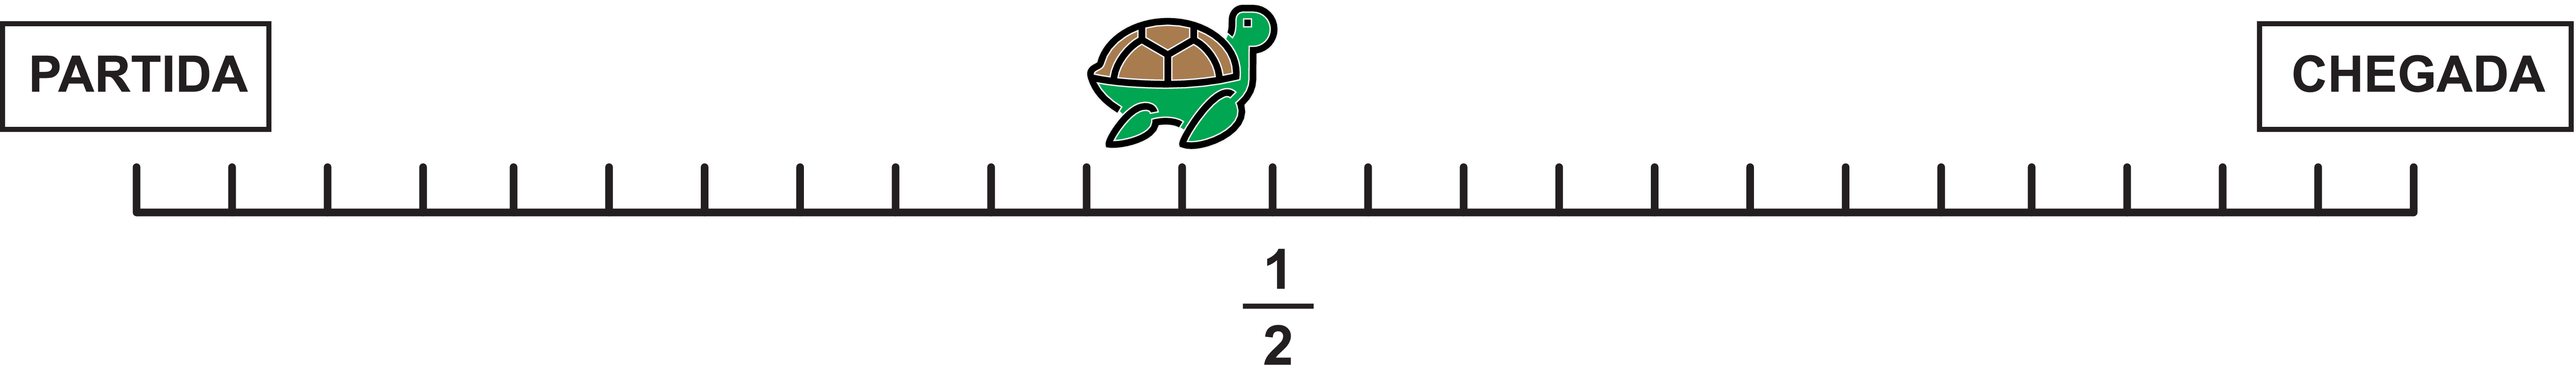
\includegraphics[width=195pt, keepaspectratio]{..//media/cap3/secoes/png/ativ9_resp_a}

\begin{enumerate} [\quad a)] %s
\item[b)]     Não está correta. Dividindo-se o percurso em quartos, como ilustra a figura a seguir, fica claro que o ponto correspondente a     $\frac{3}{4}$     do percurso está adiante da localização da tartaruga. Portanto, a tartaruga não percorreu mais do que     $\frac{3}{4}$     do percurso total.          

\end{enumerate}

 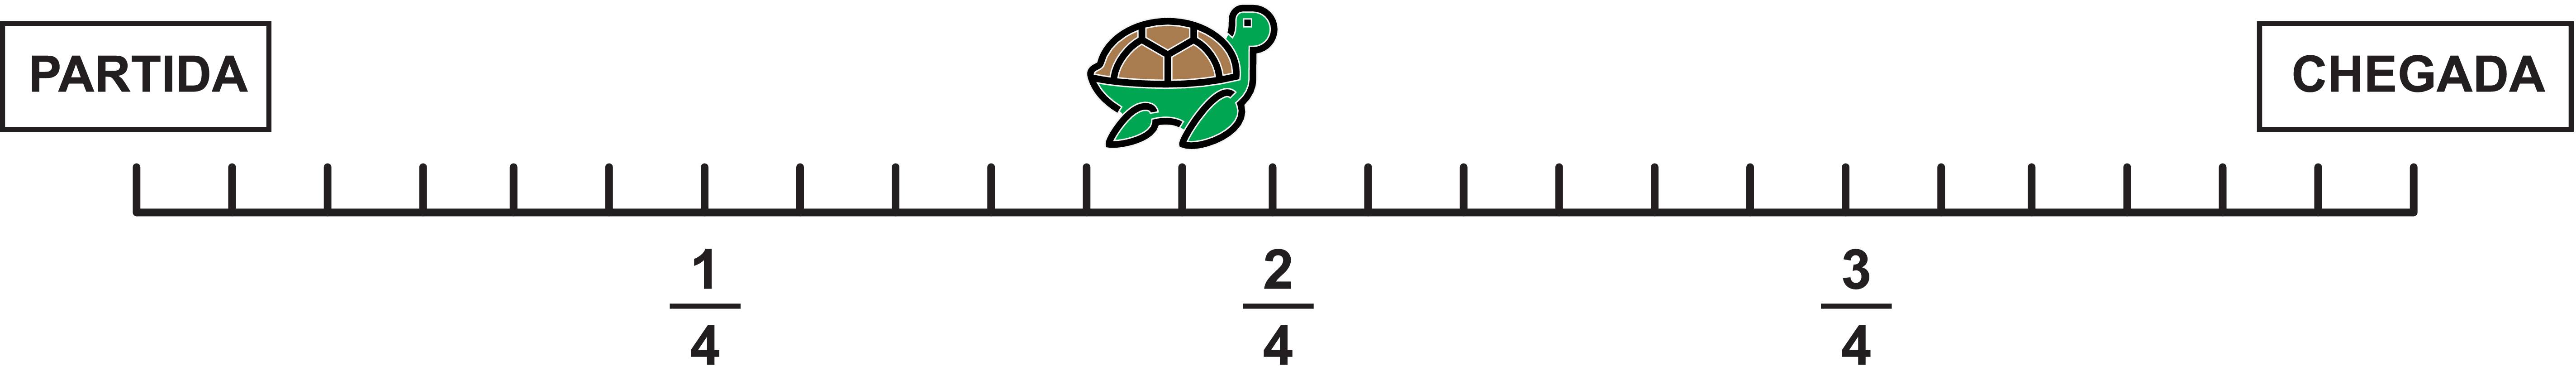
\includegraphics[width=195pt, keepaspectratio]{..//media/cap3/secoes/png/ativ9_resp_b}

\begin{enumerate} [\quad a)] %s


  \item[c)]     Está correta. Dividindo-se o percurso em oitavos, como ilustra a figura a seguir, fica claro que o ponto correspondente a     $\frac{3}{8}$     do percurso está antes da localização da tartaruga. Portanto, verifica-se que a tartaruga percorreu mais do que     $\frac{3}{8}$     do percurso total.          
\end{enumerate}

 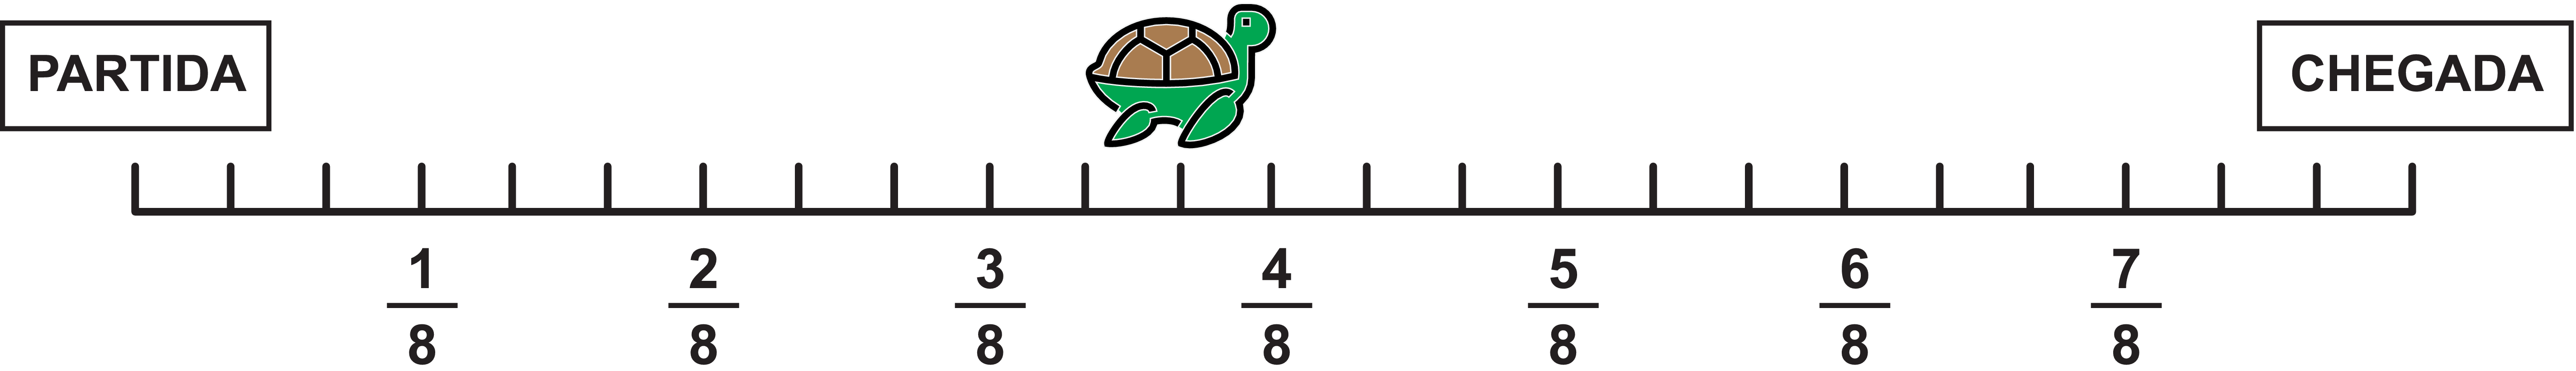
\includegraphics[width=195pt, keepaspectratio]{..//media/cap3/secoes/png/ativ9_resp_c}

\begin{enumerate} [\quad a)] %s
  \item[d)]     Está correta. Dividindo-se o percurso em quartos, como ilustra a figura a seguir, verifica-se que a localização da tartaruga é anterior ao ponto correspondente a     $\frac{3}{4}$     do percurso. Portanto, a tartaruga percorreu menos do que     $\frac{3}{4}$     do percurso total.         
\end{enumerate}

 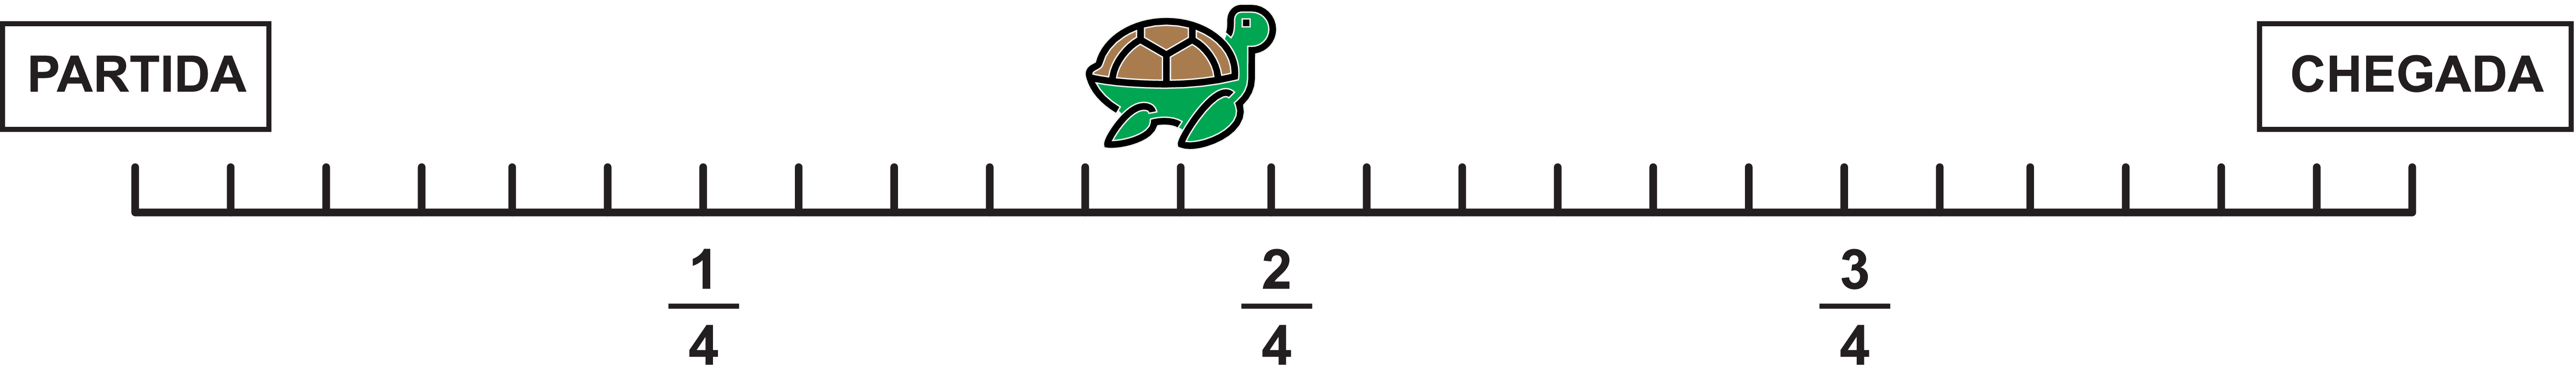
\includegraphics[width=195pt, keepaspectratio]{..//media/cap3/secoes/png/ativ9_resp_d}

\begin{enumerate} [\quad a)] %s
  \item[e)]     Não está correta. Dividindo-se o percurso em oitavos, como ilustra a figura a seguir, fica claro que o ponto correspondente a     $\frac{2}{8}$     do percurso está antes da localização da tartaruga. Portanto,verifica-se que a tartaruga percorreu mais do que     $\frac{2}{8}$     do percurso.          
\end{enumerate}

 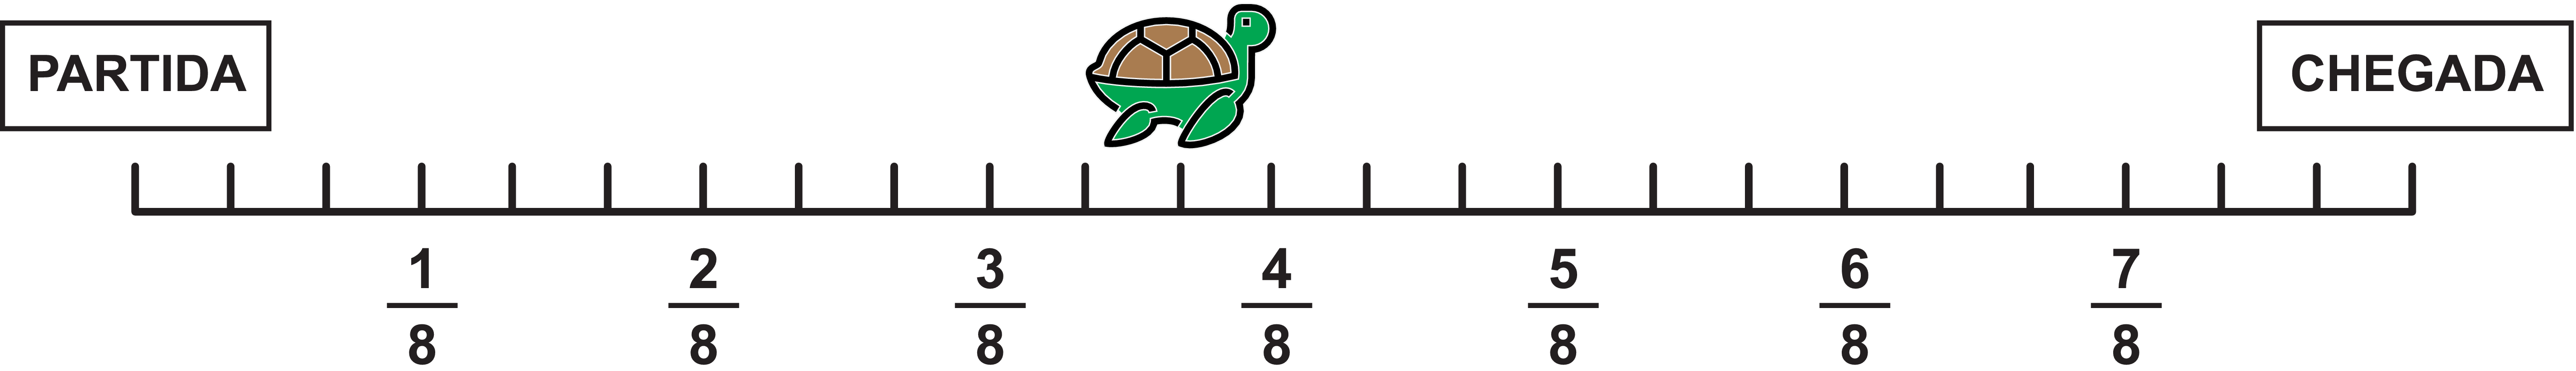
\includegraphics[width=195pt, keepaspectratio]{..//media/cap3/secoes/png/ativ9_resp_e}

\begin{enumerate} [\quad a)] %s

  \item[f)]     Está correta. Dividindo-se o percurso em terços, fica claro que o ponto correspondente a     $\frac{2}{3}$     do percurso está adiante da localização da tartaruga. Portanto, verifica-se que a tartaruga percorreu menos do que     $\frac{2}{3}$     do percurso          
\end{enumerate}

 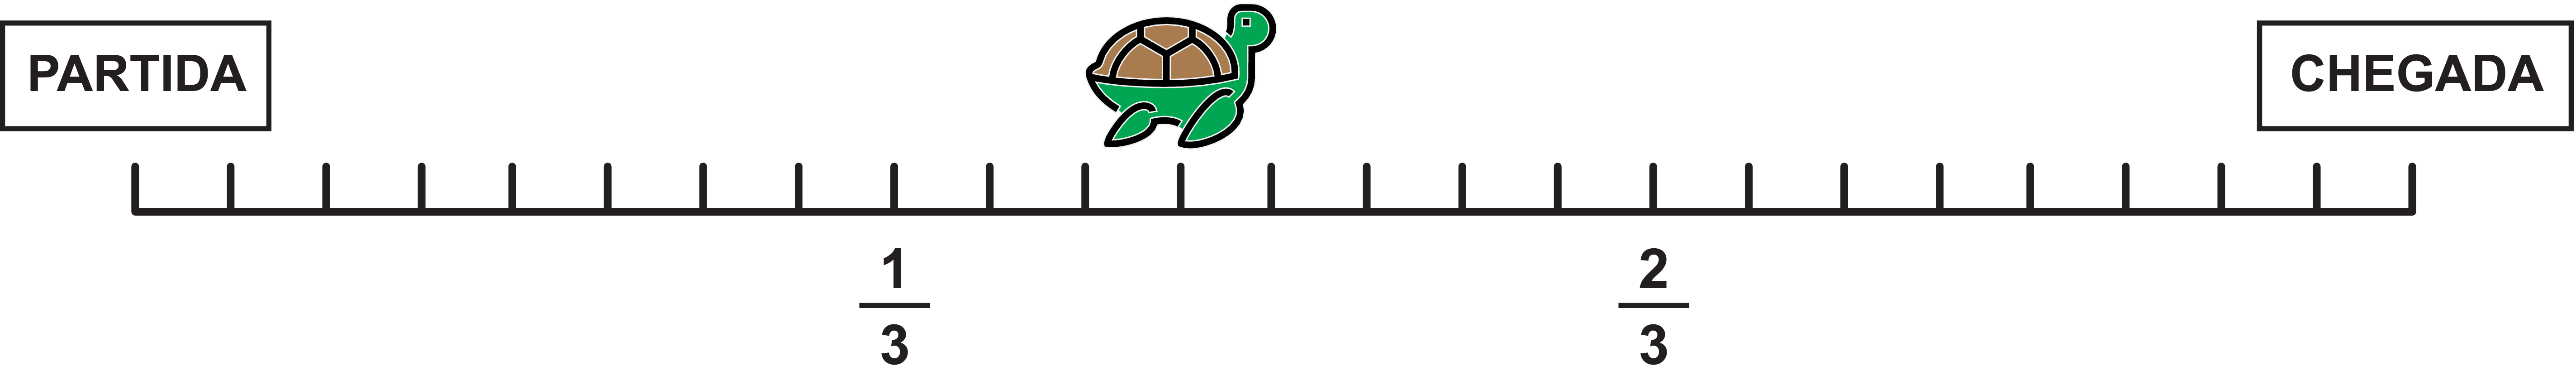
\includegraphics[width=195pt, keepaspectratio]{..//media/cap3/secoes/png/ativ9_resp_f}

\begin{enumerate} [\quad a)] %s

  \item[g)]     Não está correta. Dividindo-se o percurso em quartos, como ilustra a figura a seguir, fica claro que o ponto correspondente a     $\frac{3}{4}$     do percurso está adiante da localização da tartaruga. Portanto, verifica-se que a tartaruga percorreu menos do que     $\frac{3}{4}$     do percurso.          
\end{enumerate}

 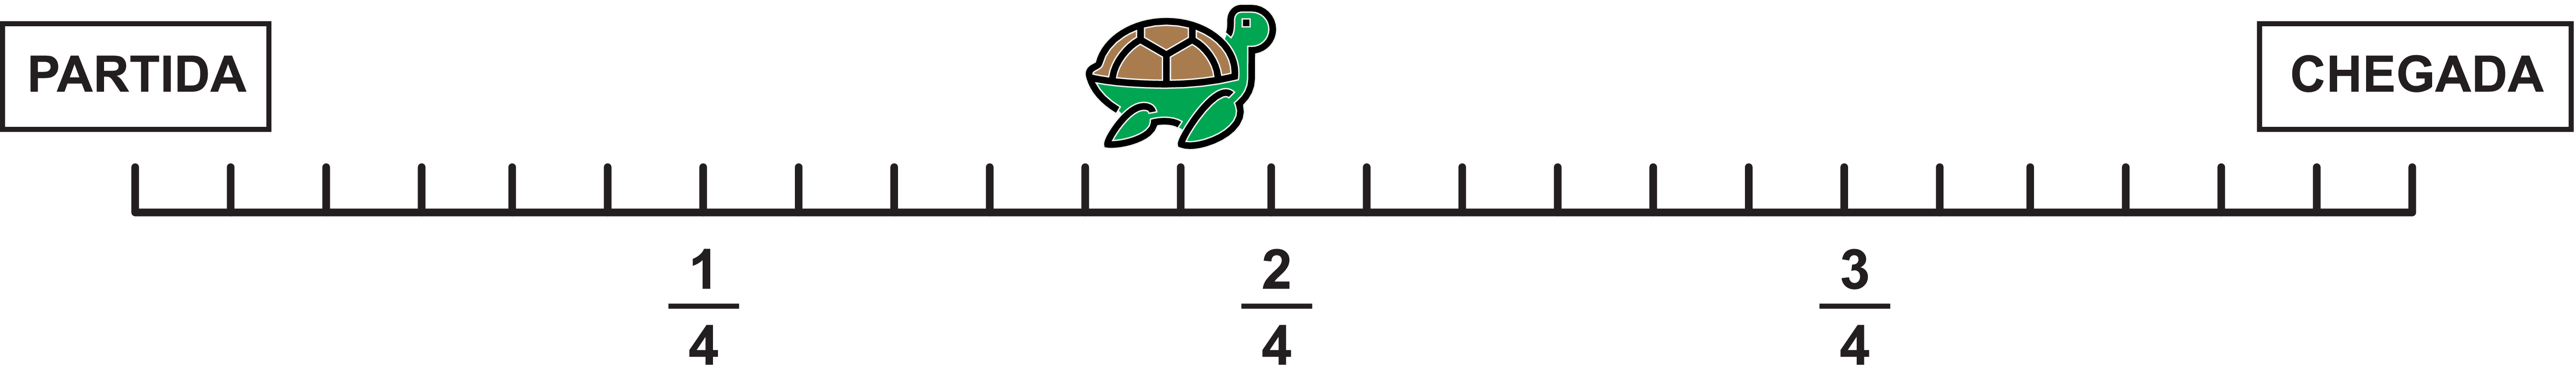
\includegraphics[width=195pt, keepaspectratio]{..//media/cap3/secoes/png/ativ9_resp_g}

\begin{enumerate} [\quad a)] %s

\item[h)]     Não está correta. Dividindo-se o percurso em oitavos, fica claro que o ponto correspondente a     $\frac{5}{8}$     do percurso está adiante da localização da tartaruga. Portanto,verifica-se que a tartaruga não alcançou     $\frac{5}{8}$     do percurso total.          
\end{enumerate}

 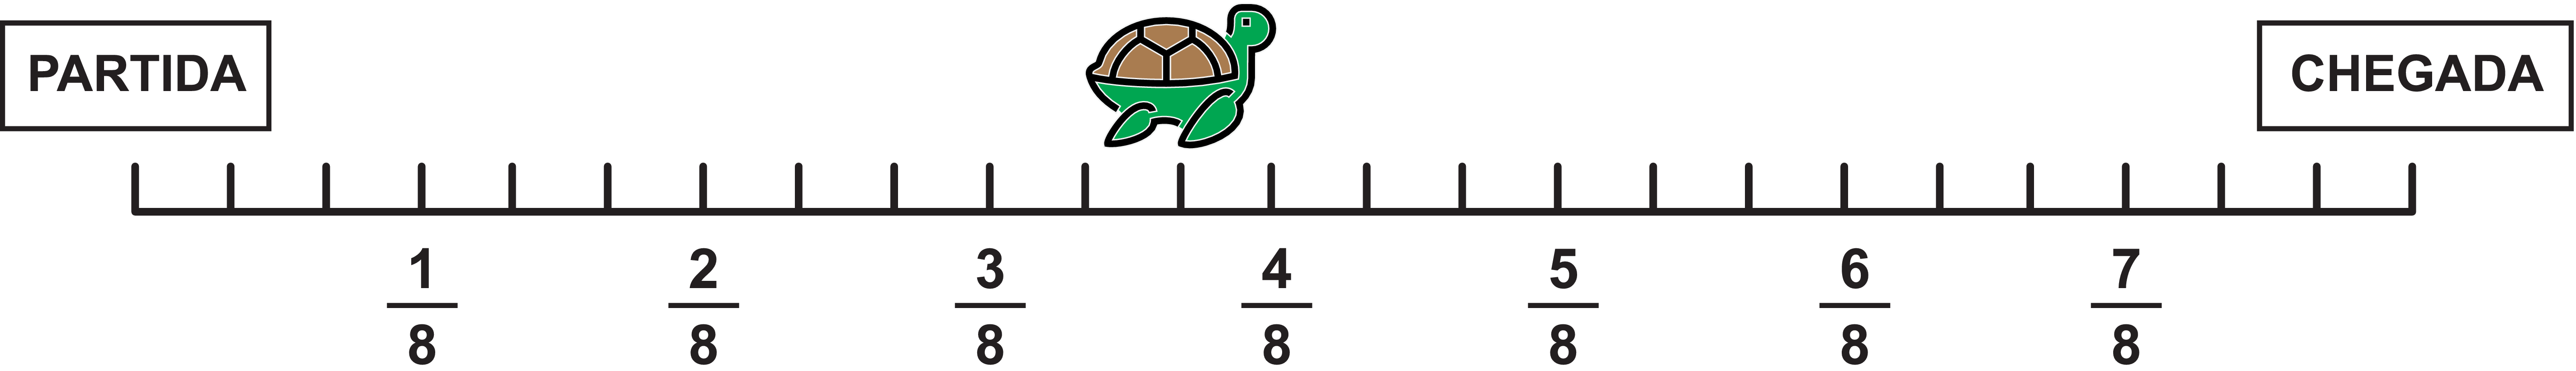
\includegraphics[width=195pt, keepaspectratio]{..//media/cap3/secoes/png/ativ9_resp_h}

\begin{enumerate} [\quad a)] %s

  \item[i)]     Está correta. De acordo com a resposta do item a), a tartaruga não alcançou a metade do percurso. Poranto, para alcançar a chegada, a tartaruga ainda precisa percorrer mais do que a metade do caminho.
  \item[j)]     Não está correta. A tartaruga já percorreu mais do que      $\frac{1}{3}$     do percurso e todo o percurso corresponde a      $\frac{3}{3}$    . Portanto, para alcançar a chegada, a tartaruga precisa percorrer menos do que     $\frac{2}{3}$     do caminho.
\end{enumerate} %s
\end{resposta*}

\subsection{Atividade 10}

\noindent {\bf Objetivos específicos: Levar o aluno a }  
\begin{itemize} %s
    \item       Representar frações na reta numérica, a partir da identificação da unidade;
    \item       Identificar, na reta numérica, os pontos correspondentes ao 0 e ao 1, a partir da represetação de duas frações (no caso, as frações       $\frac{1}{2}$       e       $\frac{3}{2}$      ).
    \item       Reconhecer a reta numérica em uma representação não comum.
\end{itemize} %s
      
\noindent {\bf Recomendações e sugestões para o desenvolvimento da atividade: }

\begin{itemize} %s
    \item       Recomenda-se que, nesta atividade, os alunos trabalhem individualmente. No entanto, é fundamental que os alunos sejam estimulados a explicar o raciocínio realizado.
    \item       Observe que a reta numérica não é apresentada da forma mais tradicional, paralela a uma das margens da página e na direção comumente chamada de horizontal. O objetivo é ampliar e variar o contato com esse modelo de representação. 
    \item       Além disso, os pontos que identificam frações da unidade (no caso, décimos) também são determinados de uma forma não tradicional. A divisão é estabelecida a partir de um feixe de retas paralelas igualmente espaçadas e transversal à reta numérica em destaque. 
    \item       Os dois primeiros itens desta atividade são bastante simples, apesar da representação não tradicional. 
    \item       O terceiro item desta atividade objetiva que o aluno identifique os pontos correspondentes ao 0 e ao 1, que determinam o segmento unitário na reta numérica, a partir dos pontos correspondentes às frações       $\frac{1}{2}$       e       $\frac{3}{2}$.  
\end{itemize} %s

\begin{resposta*}{Atividade 10}


a)

\begin{tikzpicture}[x=56.25mm,y=56.25mm, scale=.9]
 
\begin{scope}
\clip (-.2,-.2) rectangle (.85,.85); 
 
\begin{scope}[ rotate=45]
\foreach \x in {-1.1,-1,...,1.6}{
\draw[common] (\x,0) --+ (45:1); 
\draw[common] (\x,0) --+ (45:-1);}
 
\draw[attention] (-0.2,0) -- (1.2,0) ; %edit here for the axis
\foreach \x in {0,1}{ \draw (\x,3pt) -- (\x,-3pt) node[below] {\x};}
\foreach \x in {0.1,.2,...,.9}{ \draw (\x,3pt) -- (\x,-3pt);}
 
\fill[common] (.5,0) circle (3pt) node[below, black] {$\frac{1}{2}$};
 
\end{scope}
\end{scope}
 
\end{tikzpicture}   
\vspace{.5cm}
 

b)

\begin{tikzpicture}[x=56.25mm,y=56.25mm, scale=.9]
 
\begin{scope}
\clip (-.2,-.2) rectangle (.85,.85); 
 
\begin{scope}[ rotate=45]
\foreach \x in {-1.1,-1,...,1.6}{
\draw[common] (\x,0) --+ (45:1); 
\draw[common] (\x,0) --+ (45:-1);}
 
\draw[attention] (-0.2,0) -- (1.2,0) ; %edit here for the axis
\foreach \x in {0,1}{ \draw (\x,3pt) -- (\x,-3pt) node[below] {\x};}
\foreach \x in {0.1,.2,...,.9}{ \draw (\x,3pt) -- (\x,-3pt);}
 
\foreach \x in {1,2,...,9} \node[below] at (\x/10,0) {$\frac{\x}{10}$};
\fill[common] (.5,0) circle (3pt) node[above, black] {$\frac{1}{2}$};
\end{scope}
\end{scope}
 
\end{tikzpicture}   
\vspace{.5cm}
 
c)

\begin{tikzpicture}[x=56.25mm,y=56.25mm, scale=.9]
 
\begin{scope}
\clip (-.2,-.2) rectangle (.85,.85); 
 
\begin{scope}[ rotate=45]
\foreach \x in {-1.1,-1,...,1.6}{
\draw[common] (\x,0) --+ (135:1); 
\draw[common] (\x,0) --+ (135:-1);}
 
\draw[blue] (-0.2,0) -- (1.2,0) ; %edit here for the axis
\foreach \x in {0,0.1,.2,...,.9}{ \draw (\x,3pt) -- (\x,-3pt);}
\fill[common] (.2,0) circle (3pt) node[below, black] {$\frac{1}{2}$};
\fill[common] (.6,0) circle (3pt) node[below, black] {$\frac{3}{2}$};
\fill[attention] (0,0) circle (3pt) node[below, black] {0};
\fill[attention] (.4,0) circle (3pt) node[below, black] {1};
\end{scope}
\end{scope}
 
\end{tikzpicture}   
\vspace{.5cm}
 
d)
 
\begin{tikzpicture}[x=56.25mm,y=56.25mm, scale=.9]
 
\begin{scope}
\clip (-.2,-.2) rectangle (.85,.85); 
 
\begin{scope}[ rotate=45]
\foreach \x in {-1.1,-1,...,1.6}{
\draw[common] (\x,0) --+ (135:1); 
\draw[common] (\x,0) --+ (135:-1);}
 
\draw[blue] (-0.2,0) -- (1.2,0) ; %edit here for the axis
\foreach \x in {0,0.1,.2,...,.9}{ \draw (\x,3pt) -- (\x,-3pt);}
\fill[common] (.2,0) circle (3pt) node[below, black] {$\frac{1}{2}$};
\fill[common] (.6,0) circle (3pt) node[below, black] {$\frac{3}{2}$};
\fill[attention] (.3,0) circle (3pt) node[below, black] {$\frac{3}{4}$};
\fill[attention] (.5,0) circle (3pt) node[below, black] {$\frac{5}{4}$};
\end{scope}
\end{scope}
 
\end{tikzpicture}

\end{resposta*}
\vspace{-.2cm}

\subsection{Sobre o Organizando as Ideias}

Após o Organizando as Idéias, passar-se-á a falar apenas em ``fração'' ao referir-se a frações na reta numérica, subentendendo-se que já esteja claro para os alunos que trata-se de uma ``fração da unidade''. A unidade é identificada na reta pelo segmento de extremos 0 e 1, mesmo que a indicação desses pontos não esteja explicita, mas que possam ser determinados a partir de outras informações (por exemplo, as marcações das frações  $\frac{1}{2}$ e~$\frac{3}{2}$.

Espera-se que, ao longo desta lição, o aluno tenha associado fração a uma quantidade. Assim, no parágrafo que trata sobre a ordem na reta numérica, fala-se nos ``números representados na reta numérica'', incluindo-se, entre eles, as frações.
Lembre que a justaposição de segmentos pode sempre ser feita com a ajuda do compasso, evitando-se assim, medida.

\Bg
\Bg


% \begin{multicols}{2}
\subsection{Atividade 11}

\noindent {\bf Objetivos específicos: Levar o aluno a}
\begin{itemize} %s
  \item     Reconhecer a representação das frações na reta numérica;
  \item     Ordenar frações. 
\end{itemize} %s

\noindent {\bf Material necessário:}
\begin{itemize} %s
  \item     Pelo menos     $3$     metros de barbante, de maneira que cubra toda uma lateral da sala de aula (por exemplo, aquela em que está posicionado o quadro). 
  \item         $4$     folhas de papel sufite. 
  \item         $32$     pregadores de roupa (podem ser substituídos por clipes de papel).
  \item     Fita adesiva.
\end{itemize} %s

\noindent {\bf Preparação para a atividade:}
\begin{itemize} %s
  \item     Esta atividade deve ser desenvolvida como um jogo, envolvendo todos os alunos da turma, organizados em grupos com 5 ou 6 alunos. A quantidade de participantes em cada grupo e, consequentemente, a quantidade de grupos, deve ser decidida tendo em conta a quantidade de alunos na turma. Tudo deve ser combinado e esclarecido antes de a atividade começar.
  \item     O professor deve fazer um  ``varal'' com o barbante em um local que seja visível para todos os alunos e não muito alto para que os estudantes possam alcançar com as mãos. Pode ser, por exemplo, em frente ao quadro, e indo de um extremo a outro da sala. Esse barbante representará a reta numérica. 
  \item O objetivo da atividade é ``pendurar os números'' no barbante usando pregadores ou fitas adesivas, visando experimentar, em uma atividade concreta, a associação entre os pontos da reta e os números. Para isso, serão feitos cartões numerados. 
  \item É Importante reforçar a fixacão das extremidades do barbante para que não solte com o peso dos cartões que serão pendurados.
  \item Dobre cada uma das folhas de papel $2$ vezes ao meio, em direções paralelas aos lados, marcando assim 4 retângulos congruentes em cada folha. Recorte esses retângulos. Cada um deles será numerado e, durante a atividade, fixado no barbante. Serão chamados de {\bf cartões numerados} (como os da figura). 
  \item  Escreva as os números $0$, $1$, $2$, $3$, $\frac{1}{2}$, $\frac{2}{2}$, $\frac{3}{2}$, $\frac{4}{2}$, $\frac{5}{2}$, $\frac{6}{2}$, $\frac{1}{3}$, $\frac{2}{3}$, $\frac{3}{3}$, $\frac{4}{3}$, $\frac{7}{3}$, $\frac{9}{3}$, $\frac{1}{4}$, $\frac{2}{4}$, $\frac{3}{4}$, $\frac{4}{4}$, $\frac{5}{4}$, $\frac{6}{4}$, $\frac{8}{4}$, $\frac{10}{4}$, $\frac{11}{4}$, $\frac{12}{4}$, $\frac{1}{5}$, $\frac{3}{5}$, $\frac{4}{5}$, $\frac{6}{5}$, $\frac{7}{5}$, $\frac{10}{5}$, $\frac{1}{10}$ nesses cartões.
  \item Observe que são contemplados números naturais e frações não inteiras. 
  \item Além dos cartões numerados com o $0$ (zero) e o $1$ (um) , recomenda-se que haja pelo menos um cartão numerado para cada aluno. A sequência com $32$ números é uma sugestão básica. Essa sequência pode ser ampliada (ou reduzida) a partir da avaliação do professor. 
\end{itemize} %s

\noindent {\bf Recomendações e sugestões para o desenvolvimento da atividade:}
\begin{itemize}
  \item O desenvolvimento da atividade precisa ser mediado pelo professor. O processo e a discussão são importantes.
  \item As fichas com o $0$ (zero) e com o $1$ (um) devem ser presas no barbante pelo professor com fita adesiva antes do início da atividade, porque a distância entre o $0$ (zero) e o $1$ (um) terá o papel de unidade para o estudante determinar a posição dos demais cartões. {\bf Isso deve ser feito à vista dos alunos para ressaltar que a unidade é escolhida}. 
  \item Caso seja utilizado um barbante de $3$ metros, o zero pode ser posicionado bem próximo à extremidade e o número um a 90 cm à direita do zero.
  \item Combine todas as regras com os alunos.
  \item Recomenda-se que os grupos sejam identificados, por exemplo, por cores para facilitar a comunicação. Cada grupo, na sua vez de jogar, deve fixar um cartão numerado no varal e outro grupo deve avaliar se o cartão foi fixado em uma posição correta ou não.
  \item Distribua os cartões igualmente entre os grupos formados. 
  \item A correção da fixação realizada por um grupo deve ser decidida por outro grupo, podendo ser discutida com toda a turma. 
  \item Pontuacão: cada cartão numérico posicionado corretamente vale um ponto para o grupo que fixou o cartão. Cada avaliação correta vale meio ponto para o grupo que ficou responsável por ela. 
  \item Vence o jogo o grupo que, após a fixação de todos os cartões numerados no varal, tiver acumulado maior quantidade de pontos. 
  \item Em cada rodada, todos os grupos devem prender um cartão numérico no varal e avaliar a colcação feita por outro grupo. Varie as duplas de grupos que farão as ações de fixação/avaliação de cada cartão preso no varal. Assim, por exemplo, se a turma estiver organizada em $5$ grupos (Azul, Verde, Vermelho, Amarelo e Preto), com 6 alunos cada um, na prmeira rodada as duplas que farão a fixação/avaliação podem ser, por exemplo, azul/preto, verde/vermelho, vermelho/azul, amarelo/verde e preto/amarelo. Já na segunda rodada as duplas podem ser azul/amarelo, verde/preto, vermelho/verde, amarelo/azul e preto/vermelho. Planeje previamente essas associações e comunique aos alunos para não gerar discussão durante a realização. 
  \item Incentive e procure fazer, respeitando as questões pessoais, com que todos os alunos façam a fixação de pelo menos um cartão numerado no varal. 
  \item Escolha o grupo com o número $2$ para dar início ao jogo. Em seguida aquele que tiver o número 3. Claro que esses números serão mais facilmente posicionados no varal. Essa decisão pode ser uma estratégia deles no jogo. Além disso, quando já presos no varal, facilitarão a fixação dos demais. Pode acontecer de esses grupos não escolherem inicialmente esses catões. No entanto, quando esses cartões forem os escolhidos pelos respectivos grupos para serem fixados no barbante, discusta a relevância dessas referências para facilitar a fixação dos demais números, não inteiros.      
  \item Observe que alguns cartões numerados ocuparão a mesma posição na reta. Por exemplo, os numerados com $2$ e $\frac{4}{2}$. Nesses casos, recomenda-se que o segundo cartão a ser fixado seja preso no que já está no varal, sem que um esconda o outro. Sugere-se um abaixo do outro. Aproveite esses casos para discutir com os alunos que um mesmo número pode ter mais do que uma representação.
  \item Muito provavelmente as frações de denominador $2$ serão as mais fáceis de serem fixadas no varal. Em seguida, as de denominador $4$. A fixação das frações de denominadores $3$, $5$ e $10$ devem impor um pouco mais de desafio. Garanta que haja equilíbrio de dificuldade na distribuição dos cartões numerados entre os grupos.
  \item Estimule a discussão interna nos grupos para a decisão da posição de fixação de cada cartão numerado. O aluno eleito pelo grupo para prender o cartão no barbante deve explicar como decidiram por aquela posição.
  \item A atividade pode ser refeita recolhendo-se os cartões das frações do varal, colocando-os embaralhados sobre a mesa do professor com as faces voltadas para baixo e cada estudante deve ir à mesa do professor pegar um cartão e prendê-lo no varal.
  \item Uma variação desse jogo pode admitir que um grupo sugira frações para que outro grupo faça a fixação. Nesse caso, as frações podem ser escolhidas a partir de uma lista previamente estabelecida pelo professor. Recomenda-se que o grupo que escolher a fração faça a leitura e que o grupo que fizer a fixação registre simbolicamente essa fração. Dessa forma, a leitura e a escrita em representação simbólica também podem ser tratadas na atividade.
\end{itemize} %s

\begin{resposta*}{Atividade 11}

Para facilitar a visualização apresentamos a solução em duas retas.
\begin{center}
\begin{tikzpicture}[x=18mm,y=34mm]
\draw[->] (-0.1,0) -- (4,0) ; %reta anterior
\foreach \x in {0,.1,...,3.9}{ \draw (\x,1pt) -- (\x,-1pt);}
\foreach \x in {0,1,2,3} \node at (\x,-30pt) {\x}; 
\foreach \x in {1,2,3,4,5,6} {\draw[fill=attention] (\x/2, 0) circle (1pt); \node[above] at (\x/2,3pt) {$\frac{\x}{2}$};}
\foreach \x in {1,2,3,4,7,9} {\draw[fill=common] (\x/3, 0) circle (1pt); \node[below] at (\x/3,0) {$\frac{\x}{3}$};}
\end{tikzpicture}

\begin{tikzpicture}[x=18mm,y=34mm]
\draw[->] (-0.1,0) -- (4,0) ; %reta anterior
\foreach \x in {0,.1,...,3.9}{ \draw (\x,1pt) -- (\x,-1pt);}
\foreach \x in {1,2,3,4,5,6,8,10,11,12} {\draw[fill=attention] (\x/4, 0) circle (1pt); \node[above] at (\x/4,3pt) {$\frac{\x}{4}$};}
\foreach \x in {1,3,4,6,7,10} {\draw[fill=common] (\x/5, 0) circle (1pt); \node[below] at (\x/5,0) {$\frac{\x}{5}$};}
\node[above] at (.1,3pt) {$\frac{1}{10}$};
\end{tikzpicture}

\end{center}

\end{resposta*}


\subsection{Atividade 12}
  
  \noindent {\bf Objetivo específico:}   
\begin{itemize} %s
    \item       Representar frações na reta numérica.
    \item       Comparar frações.
\end{itemize} %s
  
  \noindent {\bf Recomendações e sugestões para o desenvolvimento da atividade: }
\begin{itemize}  
     \item  Recomenda-se que esta atividade seja realizada individualmente. No entanto, a discussão das resposta deve ser feita com toda a turma. Estimule seus alunos a explicarem suas respostas.  
     \item  A associação das frações aos pontos correspondentes exigirá estratégias e comparações variadas. Procure identificar e discutir as argumentações apresentadas pelos alunos.   
     \item  Todos os pontos necessários para estabelecer as associações solicitadas estão evidenciados na figura, no entanto, nem todos são imediatos.  
     \item  Inicialmente os alunos precisam identificar que as marcações em destaque identificam oitavos. Assim, por exemplo, para identificar quartos, será necessário reunir dois oitavos e para marcar   $\frac{3}{2}$   será necessário contar 12 oitavos.  
     \item  Esta atividade oferece também, de forma indireta, a oportunidade de os alunos estabelecerem comparações. Por exemplo, reconhecer que   $\frac{3}{4}$   é menor do que 1, que   $\frac{5}{4}$   é maior do que   $\frac{8}{4}$   = 2 e que   $\frac{10}{4}$   é menor do que   $\frac{10}{8}$  . Destaque e discuta essas e outras comparações com os seus alunos.   
\end{itemize}      
 
\begin{resposta*}{Atividade 12}
\noindent
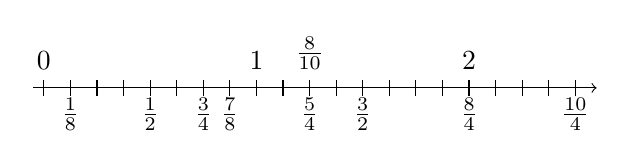
\begin{tikzpicture}[xscale=.27]
	
	\draw[->]  (-.5,0) -- (26,0);
	\draw  (0,-3pt) -- (0,3pt);
	\draw  (1.25,-3pt) -- (1.25,3pt);
	\draw  (2.5,-3pt) -- (2.5,3pt);
	\draw  (3.75,-3pt) -- (3.75,3pt);
	\draw  (5,-3pt) -- (5,3pt);
	\draw  (6.25,-3pt) -- (6.25,3pt);
	\draw  (7.5,-3pt) -- (7.5,3pt);
	\draw  (8.75,-3pt) -- (8.75,3pt);
	\draw  (10,-3pt) -- (10,3pt);
	\draw  (11.25,-3pt) -- (11.25,3pt);
	\draw  (12.5,-3pt) -- (12.5,3pt);
	\draw  (13.75,-3pt) -- (13.75,3pt);
	\draw  (15,-3pt) -- (15,3pt);
	\draw  (16.25,-3pt) -- (16.25,3pt);
	\draw  (17.5,-3pt) -- (17.5,3pt);
	\draw  (18.75,-3pt) -- (18.75,3pt);
	\draw  (20,-3pt) -- (20,3pt);
	\draw  (21.25,-3pt) -- (21.25,3pt);
	\draw  (22.5,-3pt) -- (22.5,3pt);
	\draw  (23.75,-3pt) -- (23.75,3pt);
	\draw  (25,-3pt) -- (25,3pt);

	\node[above] at (0,3pt)  {0};

	\node[below] at (5,0) {$\frac{1}{2}$};

	\node[above] at (10,3pt)  {1};

	\node[below] at (15,0) {$\frac{3}{2}$};
	
	\node[below] at (7.5,0) {$\frac{3}{4}$};

	\node[below] at (12.5,0) {$\frac{5}{4}$};
	
	\node[below] at (20,0) {$\frac{8}{4}$};

	\node[above] at (20,3pt) {2};
	
	\node[below] at (25,0) {$\frac{10}{4}$};

	\node[below] at (1.25,0) {$\frac{1}{8}$};

	\node[below] at (8.75,0) {$\frac{7}{8}$};

	\node[above] at (12.5,3pt) {$\frac{8}{10}$};
\end{tikzpicture}


\end{resposta*}


\subsection{Atividade 13}


\noindent {\bf Objetivo específico: :}
  \begin{itemize}
   \item Representação de frações $\frac{1}{d}$ na reta numérica.
   \item Comparação de frações $\frac{1}{d}$ na reta numérica.
  \end{itemize}
 

\noindent {\bf Recomendações e sugestões para o desenvolvimento da atividade:}
   \begin{itemize} 
    \item Recomenda-se que esta atividade seja realizada individualmente. No entanto, a discussão das respostas deve ser feita com toda a turma. Estimule seus alunos a explicarem suas respostas.
   \item  Observe e discuta com seus alunos que, no caso das frações de numerador igual a $1$ (frações $\frac{1}{d}$), quanto maior o denominador, menor a fração. Portanto, sua representação na reta numérica está mais perto do zero. 
   \item  Aproveite para propor e discutir com seus alunos algumas reflexões tais como: 
   \begin{enumerate}[(i)]
    \item Alguma fração com numerador igual a 1 pode ter sua representação na reta numérica entre $\frac{1}{2}$ e 1?
    \item Qual fração é maior, $\frac{1}{4}$ ou $\frac{1}{10}$?  
    \item Que fração tem sua representação na reta numérica mais próxima de 0, $\frac{1}{5}$ ou $\frac{1}{6}$?
   \end{enumerate}
 
  \end{itemize}
  

\begin{resposta*}{Atividade 13}

As respostas são na ordem I, A, B, H, F, C, E, D e G. 

\end{resposta*}

\subsection{Atividade 14}

\noindent {\bf Objetivo específico:}  Comparação de frações unitárias em sua representação simbólica.

\noindent {\bf Recomendações e sugestões para o desenvolvimento da atividade:}
\begin{itemize}
 \item  Recomenda-se que esta atividade seja realizada individualmente. No entanto, a discussão das resposta deve ser feita com toda a turma. Estimule seus alunos a explicarem suas respostas.
 \item  Esta atividade é complementar da anterior. Na atividade anterior, as frações estão representadas na reta numérica. Nesta, as frações unitárias são apresentadas em sua representação simbólica, na forma $\frac{a}{b}$. Espera-se que os alunos consigam compará-las fazendo relação com a representação na reta numérica, tratada na atividade anterior. Assim, por exemplo, a desigualdade $\frac{1}{10} < \frac{1}{4}$ pode ser justificada pelo fato de que, na representação na reta numérica, a fração $\frac{1}{10}$ está mais próxima do ponto correspondente ao zero do que a fração $\frac{1}{4}$. 
\end{itemize}

\begin{resposta*}{Atividade 14}
\begin{enumerate}[a)]
 \item $\frac{1}{2}>\frac{1}{5}$.
\item $\frac{1}{4}<\frac{1}{3}$.  
\item $\frac{1}{10}>\frac{1}{20}$. 
\item $\frac{1}{12}<\frac{1}{2}$.
\item $\frac{1}{35}>\frac{1}{43}$.
\item  $\frac{1}{99}>\frac{1}{100}$.
\item  $\frac{1}{5}>\frac{1}{50}$.
\item  $\frac{1}{100}<\frac{1}{10}$.
\end{enumerate}
 
\end{resposta*}


\subsection{Atividade 15}
  
  \noindent {\bf Objetivo específico:   }
\begin{itemize} %s
    \item       Comparação de frações com o mesmo numerador ou com o mesmo denominador, a partir de um referencial.
\end{itemize} %s
  
  
\noindent {\bf Recomendações e sugestões para o desenvolvimento da atividade: }
\begin{itemize}
    \item       Recomenda-se que esta atividade seja realizada em duplas. No entanto, a discussão das resposta deve ser feita com toda a turma.
    \item       Estimule seus alunos a explicarem suas respostas.
    \item       A associação das frações aos pontos correspondentes exigirá que os alunos saibam associar pontos na reta numérica às frações correspondentes e que façam comparações de diferentes tipos. Valorize e discuta as diversas estratégias apresentadas pelos alunos. 
    \item       Por exemplo, uma vez que os pontos correspondentes ao 0, ao 1 e a       $\frac{1}{2}$       já estão destacados, é natural que as primeiras frações a serem associadas a pontos na reta numérica sejam       $\frac{1}{4}$       e       $\frac{3}{4}$. Em seguida, reconhecendo que       $\frac{1}{8}$       corresponde à metade de       $\frac{1}{4}$,  as frações       $\frac{3}{8}$       e       $\frac{5}{8}$       podem ser as próximas.  Na sequência, o aluno pode reconhecer que       $\frac{4}{5}$       e       $\frac{9}{10}$       são menores do que a unidade e que       $\frac{9}{8}$       e       $\frac{11}{10}$       são maiores.  Entre       $\frac{4}{5}$       e       $\frac{9}{10}$,       $\frac{9}{10}$       pode ser identificada como maior por faltar  apenas       $\frac{1}{10}$       para compor a unidade , enquanto que para       $\frac{4}{5}$       falta       $\frac{1}{5}$       da unidade. Por fim, por raciocínio análogo, a fração       $\frac{9}{8}$       pode ser identificada como maior do que       $\frac{11}{10}$: Sabe-se que $\frac{1}{8}$ é maior do que $\frac{1}{10}$ e que $\frac{9}{8}$  é  $\frac{1}{8}$       maior do que a unidade, enquanto que       $\frac{11}{10}$       é        $\frac{1}{10}$       maior. Portanto, $\frac{9}{8}$    é maior do que       $\frac{11}{10}$.
    \item       Se achar necessário, discuta a comparação entre alguns pares das frações apresentadas antes de os alunos resolverem a atividade. Por exemplo, peça-lhes que comparem       $\frac{3}{8}$        e       $\frac{5}{8}$, que são frações com o mesmo denominador. Ou que comparem       $\frac{9}{8}$       e       $\frac{9}{10}$, frações com o mesmo numerador.
    \item       O aluno pode responder simplesmente       ``ligando''       os cartões com as frações aos pontos correspondentes na reta numérica. No entanto, recomenda-se que o professor oriente-os a escrever as frações abaixo dos pontos corrrespentes na reta numérica, a exemplo do 0, do 1, e de       $\frac{1}{2}$.
\end{itemize} %s
 
\begin{resposta*}{Atividade 15}

\begin{tikzpicture}
\begin{scope}[scale=.15]
	\draw  (-2,0) -- (45,0);
	\draw[->]  (45,0) -- (47,0);

	
	\node  at (0,-1) {0};						%0
	\node  at (20,-1.75) {$\frac{1}{2}$};		%1/2
	\node  at (40,-1) {1};					%1

	\node  at (10,-1.75) {$\frac{1}{4}$};			%1/4
	\node  at (15,-1.75) {$\frac{3}{8}$};			%3/8

	\node  at (25,-1.75) {$\frac{5}{8}$};			%5/8
	\node  at (30,-1.75) {$\frac{3}{4}$};			%3/4
	\node  at (32,-1.75) {$\frac{4}{5}$};			%4/5
	\node  at (36,-1.75) {$\frac{9}{10}$};			%9/10

	\node  at (43.5,-1.75) {$\frac{11}{10}$};		%11/10
	\node  at (45.5,-1.75) {$\frac{9}{8}$};			%9/8
\end{scope}
	
	\foreach \x in {0,10,15,20,25,30,32,36,40,44,45} \fill[common] (\x*.15,0) circle (2pt);

\end{tikzpicture}
  
\end{resposta*}

\subsection{Atividade 16}

\noindent {\bf Objetivo específico:}   Comparação de frações.

\noindent {\bf Recomendações e sugestões para o desenvolvimento da atividade:}
   \begin{itemize}
   \item   Recomenda-se que esta atividade seja realizada individualmente. No entanto, a discussão das respostas deve ser feita com toda a turma. Estimule seus alunos a explicarem suas respostas.
   \item Nesta atividade, as frações são apresentadas apenas em sua representação simbólica na forma $\frac{a}{b}$. Espera-se que os alunos consigam compará-las a partir da ideia de quantidade, sem necessariamente recorrer às representações em modelos contínuos ou na reta numérica. Assim, por exemplo, a comparação entre $\frac{1}{2}$ e $\frac{1}{3}$ fica estabelecida pelo fato de que a primeira identifica uma das partes da equipartição da unidade por dois, enquanto que $\frac{1}{3}$ identifica uma das partes da equipartição da mesma unidade por três. Logo, $\frac{1}{2} > \frac{1}{3}$. 
   \item No entanto, é importante observar que alguns alunos podem precisar do apoio das demais representações citadas. A discussão de cada item deve ser amparada por, pelo menos, uma das três estratégias destacadas: (i) argumentação verbal amparada pela ideia de quantidade; (ii) representação em modelos contínuos e (iii) representação na reta numérica. Por exemplo, na correção do item a), entre $\frac{3}{6}$ e $\frac{5}{6}$, espera-se que a discussão contemple:
   \begin{enumerate}[(i)]
    \item o fato de que, como essas frações indicam quantidades de ``sextos'', a menor (maior) é aquela que têm menor (maior) numerador. Portanto, $\frac{3}{6}< \frac{5}{6}$. 
    \item A representação em modelos contínuos: 
   %cap3:secoes:comparacao_sextos.jpg
    \item A representação na reta numérica %:cap3:secoes:sextos_na_reta.png.                                                                                                                                                                                                                                                                                                       
    \end{enumerate}
   
   \item Recomenda-se fortemente que os alunos sejam convidados a compartilharem com a turma as suas estratégias e que se possível, na discussão de cada item, o professor ampare a reflexão com as representações em modelos cotínuos e na reta numérica que emergirem dessa participação. No entanto, se isso não acontecer, o professor deve apresentá-las.  
   \item Observe que os primeiros itens envolvem a comparação entre frações que têm o mesmo denominador. Portanto, a comparação se estabelece a partir da comparacão entre os numeradores, amparada pelo entendimento de que quanto menor (maior) a quantidade de partes iguais, menor (maior) a fração.
   \item Os itens seguintes envolvem a comparação de frações com o mesmo numerador. Portanto, a comparação se estabelece a partir da comparação entre os numeradores, amparada pelo entendimento de que quanto maior (menor) o denominador, menor (maior) a parte da unidade.
   \item Os itens do último bloco envolvem a comparação de frações tendo a comparação dessas frações com a unidade como referência. Por exemplo, tem-se que $\frac{9}{8} > 1$. Já $\frac{9}{10} < 1$. Portanto, $\frac{9}{10}<\frac{9}{8}$.
\end{itemize}

\begin{resposta*}{Atividade 16}
\begin{enumerate}[a)]
 \item $\frac{5}{9} > \frac{4}{9}$ 
 \item $\frac{3}{6} < \frac{5}{6}$
\item   $\frac{7}{10} < \frac{9}{10}$    
\item  $\frac{3}{12} < \frac{9}{12}$    
\item $\frac{39}{100} > \frac{25}{100}$ 

\item   $\frac{1}{2} > \frac{1}{3}$     
\item  $\frac{1}{7} < \frac{1}{6}$     
\item   $\frac{2}{5} > \frac{2}{7}$    
\item   $\frac{4}{5} < \frac{4}{3}$    
\item   $\frac{12}{15} < \frac{12}{7}$ 
\item   $\frac{22}{80} > \frac{22}{90}$

\item   $\frac{3}{2} > \frac{2}{5}$    
\item   $\frac{3}{4} < \frac{6}{5}$    
\item   $\frac{7}{8} < \frac{10}{9}$   
\item   $\frac{6}{5} > \frac{12}{9}$   
\item  $\frac{4}{5}< \frac{5}{4}$     
\item  $\frac{35}{40}< \frac{30}{25}$ 
\item  $\frac{99}{100}<\frac{3}{2}$   
\end{enumerate}
\end{resposta*}


\subsection{Atividade 17}

  \noindent {\bf Objetivos específicos: Levar o aluno a } 
\begin{itemize} %s
    \item       Relacionar a representação de frações unitárias em modelo de área retangular com a representação dessas frações na reta numerada. 
\end{itemize} %s
    
  \noindent {\bf Recomendações e sugestões para o desenvolvimento da atividade: }
\begin{itemize} %s
    \item       Recomenda-se que esta atividade seja realizada em duplas ou em trios. No entanto, a discussão das respostas deve ser feita com toda a turma.
    \item       Cada aluno deve receber o material para o desenvolvimento da atividade, que consiste em uma folha, disponível para reprodução, em que há 10 retângulos congruentes, cada um com uma cor e indicando uma equipartição diferente da unidade, como ilustrado a seguir. As faixas estão subdivididas em : 2, 3, 4, 5, 6, 7, 8, 9, 10 e 16 partes iguais. 
    \item       Para o desenvolvimento da atividade, recomenda-se que os alunos cortem e manuseiem o material a ser reproduzido (veja as folhas para reprodução no final do livro). É importante que reconheçam que todas as faixas coloridas são iguais (congruentes), o que pode ser feito pela sobreposição. O retângulo representa a unidade. Além disso, é importante que percebam que cada uma das faixas (ou a unidade) tem uma equipartição indicada, representando frações unitárias diferentes. Por exemplo, cada parte da faixa amarela representa       $\frac{1}{5}$       da unidade.
    \item       No item b), observe que na imagem da reta numerada, apesar das marcações, não estão escritos os números 0 e 1. Oriente seus alunos a fazer essa identificação e a relacioná-la com a unidade considerada, o retângulo.
    \item       Algumas das frações indicadas para serem representadas na reta numérica são maiores que uma unidade. Nesses casos, oriente seus alunos a fazer a justaposição das partes dos retângulos correspndentes. Por exemplo, para representar       $\frac{12}{7}$       será necessário justapor um retângulo a cinco partes do retângulo laranja.
\end{itemize} %s

\begin{resposta*}{Atividade 17}  

a) De cima para baixo as frações são 1, $\frac{1}{2}$, $\frac{1}{3}$, $\frac{1}{4}$, $\frac{1}{5}$, $\frac{1}{6}$, $\frac{1}{7}$, $\frac{1}{8}$, $\frac{1}{9}$, $\frac{1}{10}$ e $\frac{1}{16}$
 
    
b) Para facilitar a visualização apresentamos apenas o segmento de 0 a 2 ampliado.


 \noindent \begin{tikzpicture}[x=35mm,y=35mm]
\draw[-] (0,0) -- (2,0);
\foreach \x in {0,1,2} {\draw (\x,-3pt) -- (\x,3 pt); \node at (\x,10pt) {\x};}
%\node at (60,-20pt) {1};
\foreach \x in {2,3,4} {\fill[common] (1/\x,0) circle (2 pt);\node at (1/\x,-10pt) {$\frac{1}{\x}$};}
\fill[common] (.75,0) circle (2 pt);\node at (.75,-10pt) {$\frac{3}{4}$};
\fill[common] (.6,0) circle (2 pt);\node at (.6,-10pt) {$\frac{3}{5}$};
\fill[common] (5/6,0) circle (2 pt);\node at (5/6,-10pt) {$\frac{5}{6}$};
\fill[common] (7/6,0) circle (2 pt);\node at (7/6,-10pt) {$\frac{7}{6}$};
\fill[common] (6/7,0) circle (2 pt);\node at (6/7,10pt) {$\frac{6}{7}$};
\fill[common] (10/7,0) circle (2 pt);\node at (10/7,10pt) {$\frac{10}{7}$};
\fill[common] (12/7,0) circle (2 pt);\node at (12/7,10pt) {$\frac{12}{7}$};
\fill[common] (10/8,0) circle (2 pt);\node at (10/8,-10pt) {$\frac{10}{8}$};
\fill[common] (12/8,0) circle (2 pt);\node at (12/8,-10pt) {$\frac{12}{8}$};
\fill[common] (10/9,0) circle (2 pt);\node at (10/9,10pt) {$\frac{10}{9}$};
\fill[common] (12/9,0) circle (2 pt);\node at (12/9,-10pt) {$\frac{12}{9}$};
\fill[common] (1,0) circle (2 pt);\node at (1,-10pt) {$\frac{10}{10}$};
\fill[common] (20/16,0) circle (2 pt);\node at (20/16,10pt) {$\frac{20}{16}$};
\end{tikzpicture}

 
\end{resposta*}

\subsection{Atividade 18}

  \noindent {\bf Objetivo específico:   }
\begin{itemize} %s
    \item       Representação de frações na reta numérica.
    \item       Comparação de frações a partir de sua representação na reta numérica.
\end{itemize} %s

\noindent {\bf Recomendações e sugestões para o desenvolvimento da atividade: }
\begin{itemize}
    \item       Recomenda-se que esta atividade seja realizada em duplas. No entanto, a discussão das respostas deve ser feita com toda a turma.
    \item       Estimule seus alunos a explicarem suas respostas.
    \item       A associação das frações aos pontos correspondentes exigirá que os alunos saibam associar pontos na reta numérica às frações correspondentes e que façam comparações de diferentes tipos. Valorize e discuta as diversas estratégias apresentadas pelos alunos. 
    \item       Observe que apenas os pontos correspondentes a       $0$       e a       $2$       estão destacados na reta. Ainda que não seja de fato necessário, recomenda-se que, no desenvolvimento da atividade, sejam marcados os pontos correspondentes a 1, 3, 4 e 5. Especialmente a marcação do 1, facilita a identificação da unidade.
    \item       Para a marcação de       $\frac{1}{4}$,      de $\frac{1}{2}$,   de    $\frac{3}{4}$       e   de    $\frac{5}{4}$, espera-se que os alunos utilizem os conhecimentos adquiridos nas atividades anteriores. É uma oportunidade de revisão e de avaliação do aprendizado. Não se acredita que os alunos terão dificuldade para isso. Mas é importante que o professor fique atento e, se for o caso, faça a necessária revisão. 
    \item       Observe que, nesta atividade, a partir da representação na reta, o aluno é convidado a exprimir a ordem das frações em simbologia matemática. Aproveite para destacar o fato de que quanto menor a fração, mais próxima do zero será sua representação na reta. 
    \item       Os últimos itens desta atividade admitem várias respostas. Explore as soluções dadas pelos seus alunos. Aproveite para discutir estratégias variadas de comparação. Por exemplo, decidir que       $\frac{7}{2} < \frac{11}{3} < 4$       pode ser justificado pelo fato de que para marcar o ponto correspondente a       $\frac{7}{2}$       a unidade entre 3 e 4 deve ser dividida ao meio, enquanto que, para marcar o ponto correspondente a       $\frac{11}{3}$, é necessário dividí-la em três partes iguais e tomar o mais próximo de 4. Assim, como       $\frac{1}{3} < \frac{1}{2}$, pode-se concluir que       $\frac{7}{2} < \frac{11}{3} < 4$
\end{itemize} %s
  

  
\begin{resposta*}{Atividade 18}
  
\begin{center}
\begin{tikzpicture}[x=12mm,y=15mm]
\draw[->] (-0.5,0) -- (5.5,0) ; %reta anterior
\foreach \x in {0,.25, .5, .75,1, 1.25, 2, 3, 3.5, 3.333, 11/3, 15/4, 4, 17/4, 4.5, 14/3, 5}{ \fill[common] (\x,0) circle (2pt);}
\foreach \x in {1,3,5,15,17} \node[above] at (\x/4,4pt) {$\frac{\x}{4}$};
\foreach \x in {10,11,14} \node[below] at (\x/3, -4pt) {$\frac{\x}{3}$};
\foreach \x in {1,7,9} \node[above] at (\x/2, 4pt) {$\frac{\x}{2}$};
\node[below] at (0,0) {0};
\node[below] at (1,0) {1};
\node[below] at (2,0) {2};
\node[below] at (3,0) {3};
\node[below] at (4,0) {4};
\node[below] at (5,0) {5};

\end{tikzpicture}
\end{center}
  
  
\begin{enumerate} [\quad a)] %s
    \item       Uma forma de marcar       $\frac{1}{2}$       na reta numérica dada pode ser a partir da marcação, primeiro, do 1. A marcação do 1 fica entre 0 e 2, bem no meio. Com a unidade identificada, a       $\frac{1}{2}$        fica entre as marcações do 0 e do 1, bem no meio.   
    \item       As marcações de       $\frac{1}{4}$,       $\frac{3}{4}$       e       $\frac{5}{4}$       podem ser feitas de maneira semelhante, lembrando que       $\frac{1}{4}$       fica.
    \item             $\frac{1}{4}$       é menor do que       $\frac{1}{2}$       porque está mais próximo de zero.
    \item             $\frac{3}{4}$       é maior do que        $\frac{1}{2}$       porque está mais distante de zero.
    \item             $\frac{5}{4}$       é menor do que 1 porque está mais distante de zero.
    \item       Escreva as frações marcadas na reta em ordem crescente, completando os espaços a seguir:
  $$0 < \frac{1}{4} < \frac{1}{2}< \frac{3}{4} < 1 < \frac{5}{4} < 2$$     
    \item       Há várias respostas possíveis. Por exemplo,       $3 < \frac{7}{2} < 4$,       $3 < \frac{15}{4} < 4$         ou         $3 < \frac{10}{3} < 4$
    \item       Há várias respostas possíveis. Por exemplo,       $\frac{7}{2} < \frac{15}{4} < 4$ ou $\frac{7}{2} < \frac{11}{3} < 4$.
    \item       Há várias respostas possíveis. Por exemplo,       $\frac{17}{4} < \frac{9}{2} < 5$, $\frac{17}{4} < \frac{19}{4} < 5$ ou $\frac{17}{4} < \frac{14}{3} < 5$.
\end{enumerate} %s
  
  
\end{resposta*}



\end{multicols}
